\fenicschapter{Common and unusual finite elements}
              {Common and unusual finite elements}
              {Common and unusual finite elements}
              {Robert C. Kirby, Anders Logg, Marie E. Rognes and Andy R. Terrel}
              {kirby-6}

\newcommand{\elmfig}[1]{\includegraphics[width=2.0cm]{chapters/kirby-6/png/#1.png}}
\newcommand{\elmdesc}[1]{\begin{minipage}{4cm} #1 \end{minipage} \\}

This chapter provides a glimpse of the considerable range of finite
elements in the literature. Many of the elements presented here are
implemented as part of the FEniCS project already; some are future work.
The universe of finite elements extends far beyond what we consider
here. In particular, we consider only simplicial, polynomial-based
elements. We thus bypass elements defined on quadrilaterals and hexahedra,
composite and macro-element techniques, as well as XFEM-type methods. Even
among polynomial-based elements on simplices, the list of elements can be
extended. Nonetheless, this chapter presents a comprehensive collection
of some of the most common, and some more unusual, finite elements.

%------------------------------------------------------------------------------
\section{The finite element definition}

The Ciarlet definition of a \emph{finite element} was first introduced
in a set of lecture notes by \citet{Ciarlet1975} and became popular
after his 1978 book \citep{Ciarlet2002}. It remains the standard
definition today, see for example \citet{BrennerScott2008}. The
definition, which was also presented in Chapter~\ref{chap:kirby-7},
reads as follows:
%%
\begin{definition}[Finite element~{\citep{Ciarlet2002}}]
  A finite element is defined by a triple
  $(T, \CiarletSpace,\mathcal{L})$, where
  \femdefinition{}
\end{definition}
%%
Similar ideas were introduced earlier in
\citet{CiarletRaviart1972}\footnote{The Ciarlet triple was originally
  written as~$(K, P, \Sigma)$ with $K$ denoting $T$, P denoting $\CiarletSpace$, and $\Sigma$
  denoting~$\mathcal{L}$.}, in which unisolvence\footnote{To check
  whether a given set of linear functionals is a basis for
  $\CiarletSpace'$, one may check whether it is \emph{unisolvent} for
  $\CiarletSpace$; that is, for $v \in \CiarletSpace$, $\ell_i(v) = 0$
  for $i = 1, \dots, n$ if and only if $v = 0$.} of a set of
interpolation points $\{x^i\}_i$ was discussed. This is closely
related to the unisolvence of~$\mathcal{L}$ when the degrees of
freedom are given by by $\ell_i(v) = v(x^i)$.  Conditions for uniquely
determining a polynomial based on interpolation of function values and
derivatives at a set of points was also discussed in
\citet{BrambleZlamal1970}, although the term unisolvence was not used.

For any finite element, one may define a local basis for
$\CiarletSpace$ that is dual to the degrees of freedom. Such a basis
$\{\phi^T_1,\phi^T_2 \ldots , \phi^T_{n} \}$ satisfies $ \ell_i(
\phi^T_j ) = \delta_{ij} $ for $1 \leqslant i,j \leqslant n $ and is called
the \emph{nodal basis}. It is typically this basis that is used in
finite element computations.

Also associated with a finite element is a \emph{local interpolation
  operator}, sometimes called a \emph{nodal interpolant}. Given some
function $f$ on $T$, the nodal interpolant is defined by
\begin{equation}
  \Pi_T(f) = \sum_{i=1}^{n} \ell_i(f) \phi^T_i,
\end{equation}
assuming that $f$ is smooth enough for all of the degrees of freedom
acting on it to be well-defined.

Once a local finite element space is defined, it is relatively
straightforward to define a global finite element space over a
tessellation $\mathcal{T}_h$.  One defines the global space to consist
of functions whose restrictions to each $T \in \mathcal{T}_h$ lie in
the local space $\CiarletSpace(T)$ and that also satisfy any required
continuity requirements.  Typically, the degrees of freedom for each
local element are chosen such that if the degrees of freedom on a
common interface between two adjacent cells $T$ and $T'$ agree, then a
function will satisfy the required continuity condition.

When constructing a global finite element space, it is common to
construct a single \emph{reference finite element} $(\hat{T},
\hat{\CiarletSpace}, \hat{\mathcal{L}})$ and map it to each cell in
the mesh. As we are dealing with a simplicial geometry, the mapping
between $\hat{T}$ and each $T \in \mathcal{T}_h$ will be
affine. Originally defined for the purpose of error estimation, but
also useful for computation, is the notion of \emph{affine
  equivalence}. Let $F_T: \hat{T} \rightarrow T$ denote this affine
map. Let $v \in \CiarletSpace$. The \emph{pullback} associated with
the affine map is given by $\mathcal{F}^*(v)(\hat{x}) =
v(F_T(\hat{x}))$ for all $\hat{x} \in \hat{T}$. Given a functional
$\hat{\ell} \in \hat{\CiarletSpace}'$, its \emph{pushforward} acts on
a function in $v \in \CiarletSpace$ by $\mathcal{F}_*(\hat{\ell})(v) =
\hat{\ell}(\mathcal{F}^*(v))$.
%%
\begin{definition}[Affine equivalence]
  Let $(\hat{T}, \hat{\CiarletSpace}, \hat{\mathcal{L}})$ and
  $(T, \CiarletSpace, \mathcal{L})$ be finite elements and $F_T:
  \hat{T} \rightarrow T$ be a non-degenerate affine map. The finite
  elements are \emph{affine equivalent} if
  $\mathcal{F}^*(\CiarletSpace) = \hat{\CiarletSpace}$ and
  $\mathcal{F}_*(\hat{\mathcal{L}}) = \mathcal{L}$.
\end{definition}
One consequence of affine equivalence is that only a single nodal
basis needs to be constructed, and then it can be mapped to each cell
in a mesh. Moreover, this idea of equivalence can be extended to some
vector-valued elements when certain kinds of Piola mappings are used.
In this case, the affine map is the same, but the pull-back and
push-forward are appropriately modified.  It is also worth stating
that not all finite elements generate affine equivalent or
Piola-equivalent families. The Lagrange elements are affine equivalent
in $H^1$, but the Hermite and Argyris elements are not. The
Raviart--Thomas elements are Piola-equivalent in $\Hdiv$, while the
Mardal--Tai--Winther elements are not.

A dictionary of the finite elements discussed in this chapter is
presented in Table~\ref{kirby-6:tab:overview}.
\begin{table}
  \centering
  \begin{tabular}{cccc}
    \toprule
    Finite element & Short name & Sobolev space & Conforming\\
    \midrule
    (Quintic) Argyris & $\mathrm{ARG}$ & $H^2$ &Yes \\
    Arnold--Winther & $\mathrm{AW}$ & $H(\mathrm{div}; \mathbb{S})$ &Yes \\
    Brezzi--Douglas--Marini & $\mathrm{BDM}$ & $\Hdiv$ & Yes \\
    Crouzeix--Raviart & $\mathrm{CR}$ & $H^1$ & No \\
    Discontinuous Lagrange & $\mathrm{DG}$ & $L^2$ & Yes \\
    (Cubic) Hermite & $\mathrm{HER}$ & $H^2$ & No \\
    Lagrange & $\mathrm{CG}$ & $H^1$ & Yes \\
    Mardal--Tai--Winther & $\mathrm{MTW}$ & $H^1/\Hdiv$ & No/Yes \\
    (Quadratic) Morley & $\mathrm{MOR}$ & $H^2$ & No \\
    \nedelec{} first kind & $\mathrm{NED^1}$ & $\Hcurl$ & Yes \\
    \nedelec{} second kind & $\mathrm{NED^2}$ & $\Hcurl$ & Yes \\
    Raviart--Thomas & $\mathrm{RT}$ & $\Hdiv$ & Yes \\
    \bottomrule
  \end{tabular}
  \caption{A dictionary of the finite elements discussed in this
    chapter, including full name and the respective (highest order)
    Sobolev space to which the elements are conforming/nonconforming.}
  \label{kirby-6:tab:overview}
\end{table}

%------------------------------------------------------------------------------
\section{Notation}

\begin{itemize}
\item
  The space of polynomials of degree up to and including $q$ on a
  domain $T \subset \R^d$ is denoted by $\Poly{q}(T)$ and the
  corresponding $d$-vector fields by $[\Poly{q}(T)]^d$.
\item
  A finite element space $E$ is called $V$-conforming if $E \subseteq
  V$. If not, it is called ($V$-) nonconforming.
\item The elements of $\mathcal{L}$ are usually referred to as the
  \emph{degrees of freedom} of the element~$(T, \CiarletSpace,
  \mathcal{L})$. When describing finite element families, it is usual
  to illustrate the degrees of freedom with a certain schematic
  notation. We summarize the notation used here in the list below and
  in Figure~\ref{kirby-6:fig:notation}.
  \begin{description}
  \item[Point evaluation.]
    A black sphere (disc) at a point $x$ denotes point
    evaluation of the function $v$ at that point:
    \begin{equation}
      \ell(v) = v(x).
    \end{equation}
    For a vector valued function~$v$ with~$d$ components, a black
    sphere denotes evaluation of all components and thus corresponds
    to~$d$ degrees of freedom.
  \item[Evaluation of all first derivatives.]
    A dark gray, slightly larger sphere (disc) at a point $x$ denotes point
    evaluation of all first derivatives of the function $v$ at that point:
    \begin{equation}
      \ell_i(v) = \frac{\partial v(x)}{\partial x_i}, \quad i
      =1, \ldots, d,
    \end{equation}
    thus corresponding to $d$ degrees of freedom.
  \item[Evaluation of all second derivatives.]
    A light gray, even larger sphere (disc) at a point $x$ denotes point
    evaluation of all second derivatives of the function $v$ at that point:
    \begin{equation}
      \ell_{ij}(v) = \frac{\partial^2 v(x)}{\partial x_i \partial
        x_j}, \quad 1 \leqslant i \leqslant j \leqslant d,
    \end{equation}
    thus corresponding to $d (d + 1) / 2$ degrees of freedom.
  \item[Evaluation of directional component.]
    An arrow at a point $x$ in a direction $n$ denotes evaluation of
    the vector-valued function $v$ in the direction $n$ at the point
    $x$:
    \begin{equation}
      \ell(v) = v(x) \cdot n.
    \end{equation}
    The direction $n$ is typically the normal direction of a facet, or
    a tangent direction of a facet or edge. We will sometimes use an
    arrow at a point to denote a moment (integration against a weight
    function) of a component of the function over a facet or edge.
  \item[Evaluation of directional derivative.]
    A black line at a point $x$ in a direction $n$ denotes evaluation
    of the directional derivative of the scalar function $v$ in the
    direction $n$ at the point $x$:
    \begin{equation}
      \ell(v) = \nabla v(x) \cdot n.
    \end{equation}
  \item[Evaluation of interior moments.]  A set of concentric spheres
    (discs) denotes interior moment degrees of freedom; that is,
    degrees of freedom defined by integration against a weight
    function over the interior of the domain~$T$. The spheres are
    colored white-black-white etc.
  \end{description}
\end{itemize}

\begin{figure}
\bwfig
 % \centering
 \fenicsfig{kirby-6}{notation_new}{\smallfig}
 % \fenicsfig{kirby-6}{}{\smallfig}
  \caption{Summary of notation used for degrees of freedom. In this
    example, the three concentric spheres indicate a set of three
    degrees of freedom defined by interior moments.}
  \label{kirby-6:fig:notation}
\vspace*{8pt}
\end{figure}

We note that, for some of the finite elements presented below, the
literature will use different notation and numbering schemes, so that
our presentation may be quite different from the original presentation
of the elements. In particular, the families of Raviart--Thomas and
\nedelec{} spaces of the first kind are traditionally numbered
from~$0$, while we have followed the more recent scheme from the
finite element exterior calculus of numbering from~$1$.

\vspace*{7pt}
%------------------------------------------------------------------------------
\section{$H^1$ finite elements}

The space $H^1$ is fundamental in the analysis and discretization of
weak forms for second-order elliptic problems, and finite element
subspaces of $H^1$ give rise to some of the best-known finite
elements. Typically, these elements use $C^0$ approximating spaces,
since a piecewise smooth function on a bounded domain is $H^1$ if and
only if it is continuous \citep[Theorem 5.2]{Braess2007}. We consider
the classic Lagrange element, as well as a nonconforming example, the
Crouzeix--Raviart space. It is worth noting that the Hermite element
considered later is technically only an $H^1$ element, but can be used
as a nonconforming element for smoother spaces.  Also, smoother
elements such as Argyris may be used to discretize $H^1$, although
this is less common in practice.

\vspace*{7pt}
\subsection{The Lagrange element}

The best-known and most widely used finite element is the $\Poly{1}$
Lagrange element. This lowest-degree triangle is sometimes called the
\emph{Courant} triangle, after the seminal paper by \citet{Courant1943}
in which variational techniques are used with the $\Poly{1}$ triangle
to derive a finite difference method. Sometimes this is viewed as
``the'' finite element method, but in fact there is a whole family of
elements parametrized by polynomial degree that generalize the
univariate Lagrange interpolating polynomials to simplices, boxes, and
other shapes. The Lagrange elements of higher degree offer higher
order approximation properties. Moreover, these can alleviate locking
phenomena observed when using linear elements or give improved
discrete stability properties; see \citet{TaylorHood1973,
  ScottVogelius1985}.

\begin{definition}[Lagrange element]
  The Lagrange element ($\mathrm{CG}_q$) is defined for $q = 1, 2,
  \dots$ by
  \begin{align}
    T &\in \{ \mathrm{interval}{},
              \mathrm{triangle}{},
              \mathrm{tetrahedron}{}\}, \\
    \CiarletSpace &= \Poly{q}(T), \\
    \ell_i(v) &= v(x^i), \quad i = 1, \dots, n(q),
  \end{align}
  where $\{ x^i \}_{i=1}^{n(q)}$ is an enumeration of points in $T$
  defined by
  \begin{equation}
    x =
    \left \{
    \begin{array}{lll}
      i/q,             & 0 \leqslant i \leqslant q,         & T~\mathrm{interval}{}, \\
      (i/q, j/q),      & 0 \leqslant i + j \leqslant q,     & T~\mathrm{triangle}{}, \\
      (i/q, j/q, k/q), & 0 \leqslant i + j + k \leqslant q, & T~\mathrm{tetrahedron}{}.
    \end{array}
    \right.
  \end{equation}
\end{definition}
The dimension of the Lagrange finite element thus corresponds to the
dimension of the complete polynomials of degree $q$ on $T$ and is
\begin{equation}
  n(q) =
    \left \{
    \begin{array}{ll}
      q + 1, & T~\mathrm{interval}, \\
      \frac{1}{2} (q + 1)(q + 2), & T~\mathrm{triangle}, \\
      \frac{1}{6} (q + 1)(q + 2)(q + 3), & T~\mathrm{tetrahedron}.
    \end{array}
    \right.
\end{equation}

\begin{figure}
  \ffigbox{\caption{The linear Lagrange interval, triangle and tetrahedron.}
           \label{kirby-6:fig:lagrange:dim}}
  {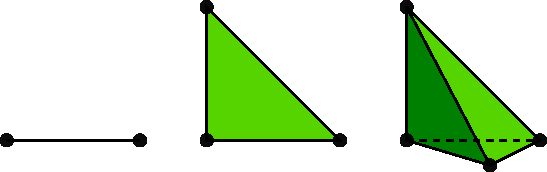
\includegraphics[width=\fullfig]{chapters/kirby-6/pdf/P1_1d2d3d.pdf}}
  %{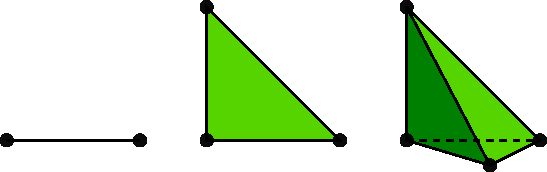
\includegraphics[width=\fullfig]{chapters/kirby-6/pdf/P1_1d2d3d.pdf}}
\end{figure}


The definition above presents one choice for the set of points
$\{x^i\}$. However, this is not the only possible choice. In general,
it suffices that the set of points $\{x^i\}$ is unisolvent and that
the boundary points are located so as to allow $C^0$ assembly. The
point set must include the vertices, $q-1$ points on each edge,
$\frac{(q-1)(q-2)}{2}$ points per face, and so forth. The boundary
points should be placed symmetrically so that the points on adjacent
cells match. While numerical conditioning and interpolation properties
can be dramatically improved by choosing these points in a clever way
\citep{Warburton2005}, for the purposes of this chapter the points
may be assumed to lie on an equispaced lattice;
see~Figures~\ref{kirby-6:fig:lagrange:dim},
\ref{kirby-6:fig:lagrange:2d} and \ref{kirby-6:fig:lagrange:3d}.

Letting $\Pi_T^q$ denote the interpolant defined by the above degrees
of freedom of the Lagrange element of degree~$q$, we have
from \citet{BrennerScott2008} that
\begin{equation}
  ||u - \Pi_T^q u||_{H^1(T)} \leqslant C \, h_T^{q} |u|_{H^{q+1}(T)}, \quad
  ||u - \Pi_T^q u||_{L^2(T)} \leqslant C \, h_T^{q+1} |u|_{H^{q+1}(T)}.
\end{equation}
where, here and throughout, $C$ denotes a generic positive constant
not depending on $h_T$ but depending on the degree $q$ and the aspect
ratio of the simplex, and $u$ is a sufficiently regular function (or
vector-field).

Vector-valued or tensor-valued Lagrange elements are usually constructed
by using a Lagrange element for each component.

\subsection{The Crouzeix--Raviart element}

{The Crouzeix--Raviart element was introduced in
\citet{CrouzeixRaviart1973} as a technique for solving the stationary
Stokes equations. The global element space consists of piecewise linear\hfilneg}



\begin{figure}
  \ffigbox{\caption{The Lagrange $\mathrm{CG}_{q}$ triangle for $q = 1,2,3,4,5,6$.}
           \label{kirby-6:fig:lagrange:2d}}
  {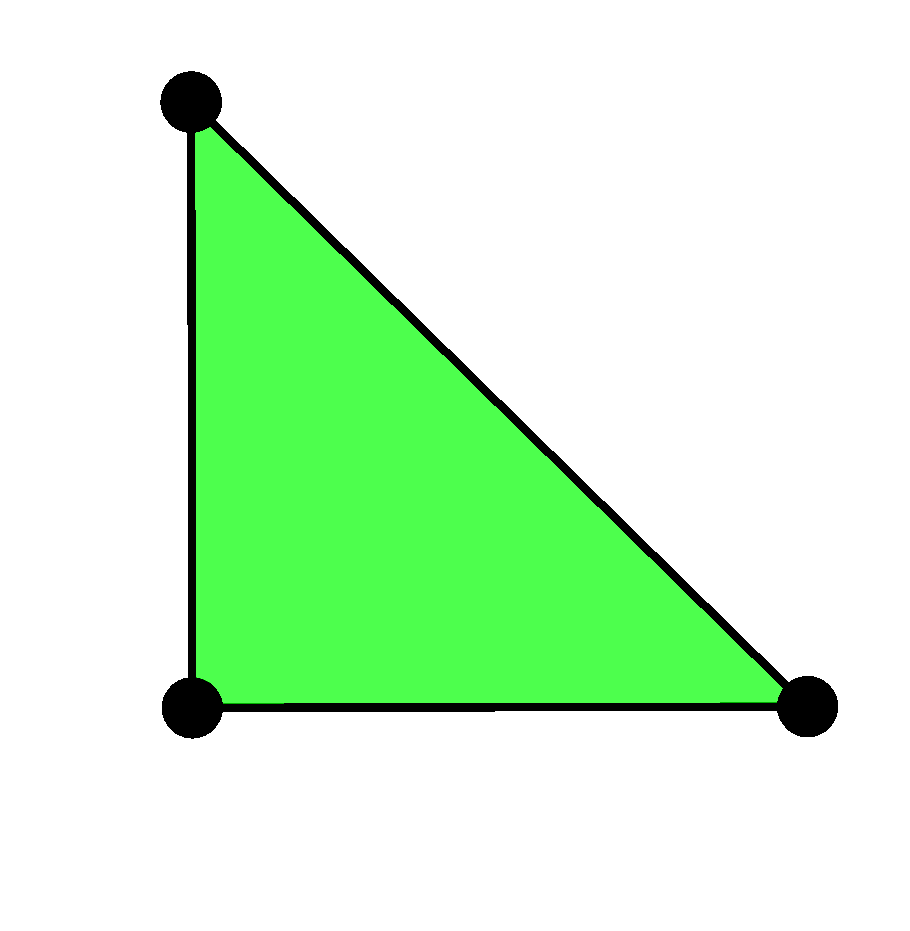
\includegraphics[width=\threefigsfull]{chapters/kirby-6/png/CG1_2d.png}
   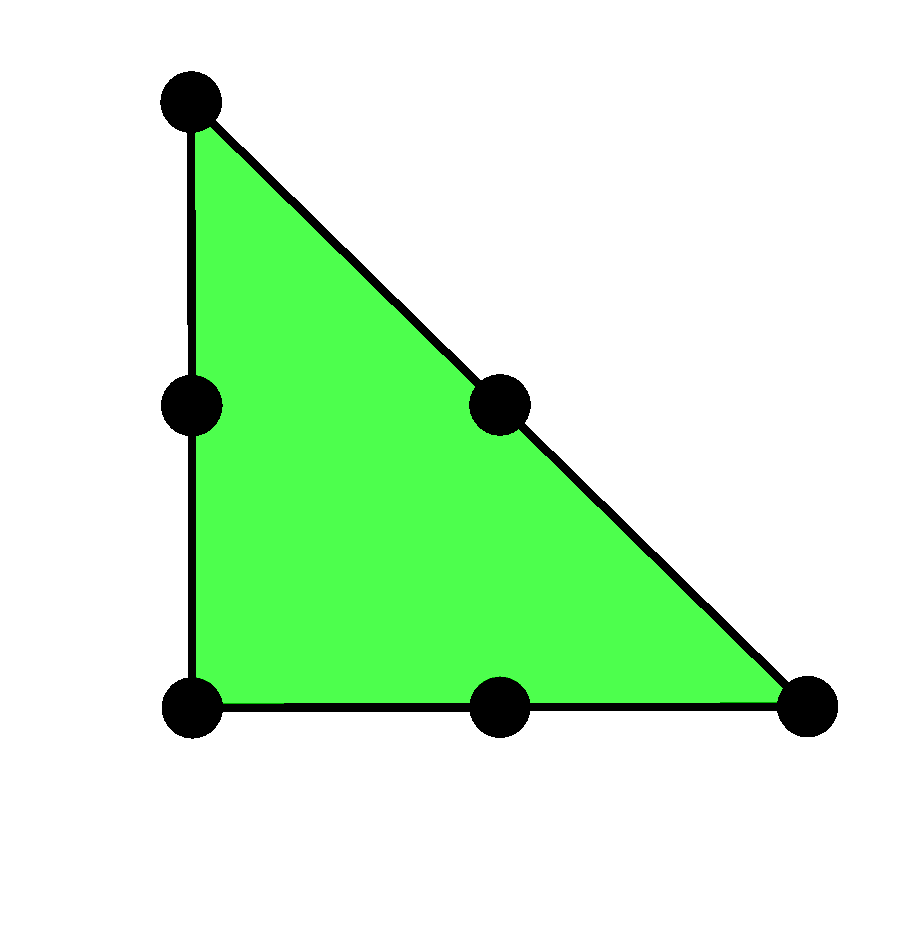
\includegraphics[width=\threefigsfull]{chapters/kirby-6/png/CG2_2d.png}
   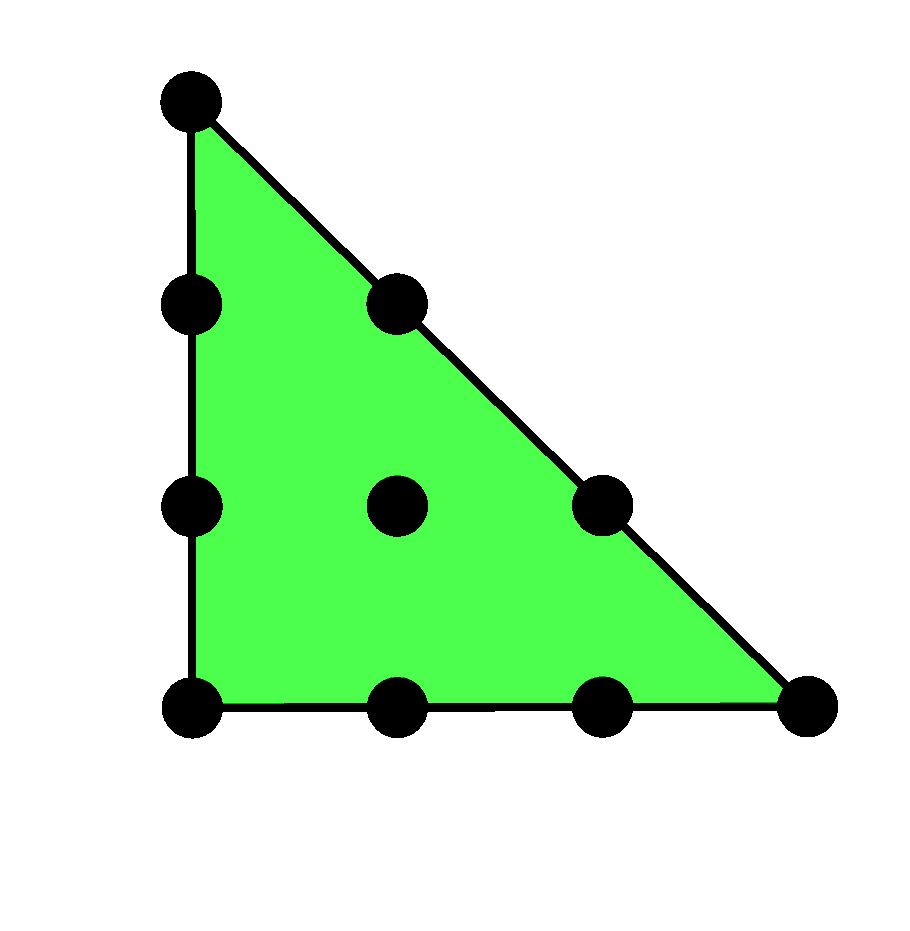
\includegraphics[width=\threefigsfull]{chapters/kirby-6/png/CG3_2d.png} \\
   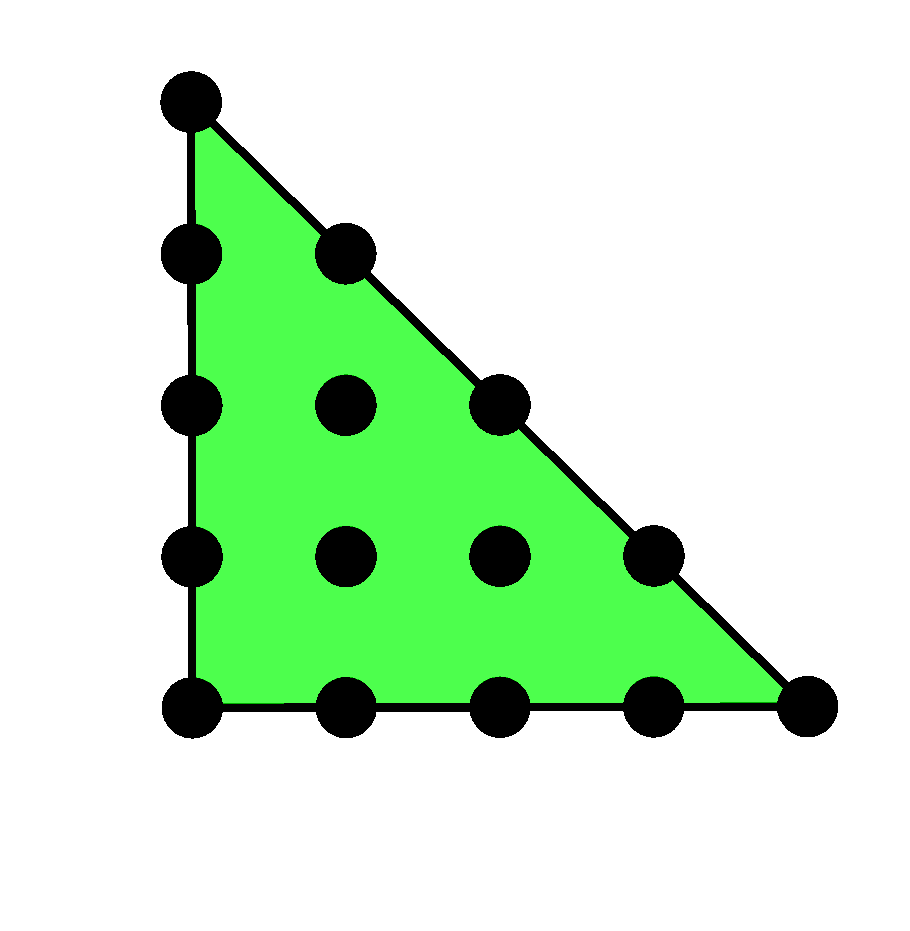
\includegraphics[width=\threefigsfull]{chapters/kirby-6/png/CG4_2d.png}
   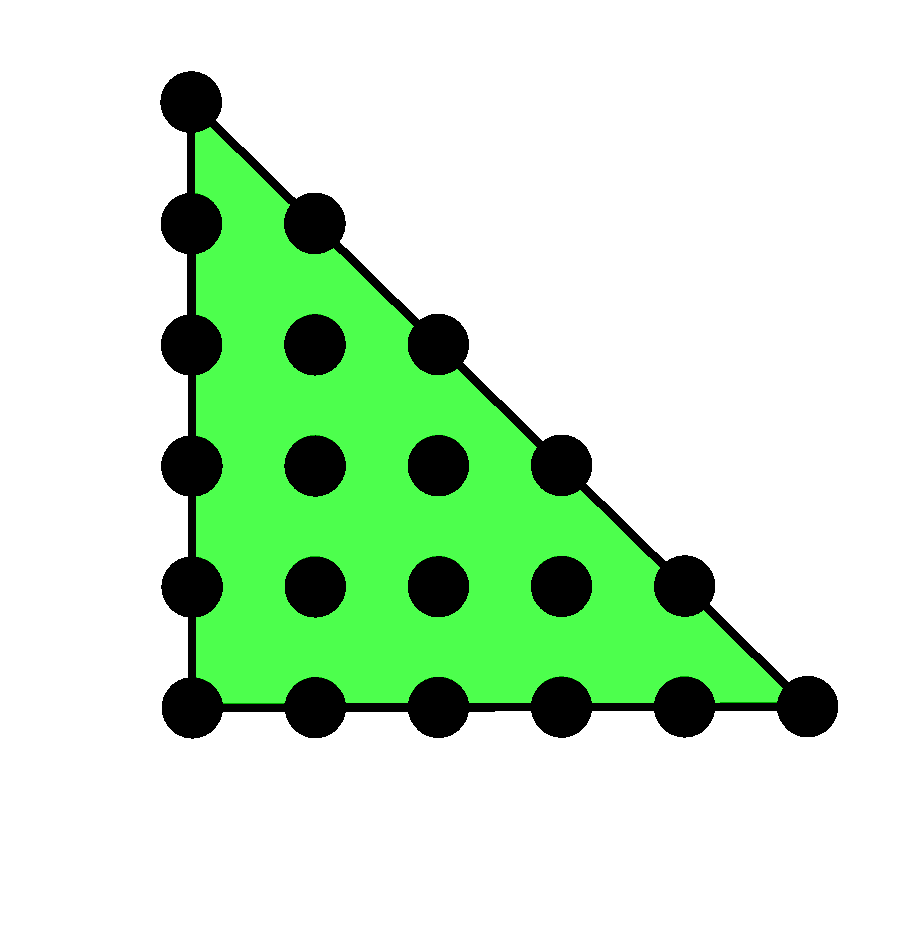
\includegraphics[width=\threefigsfull]{chapters/kirby-6/png/CG5_2d.png}
   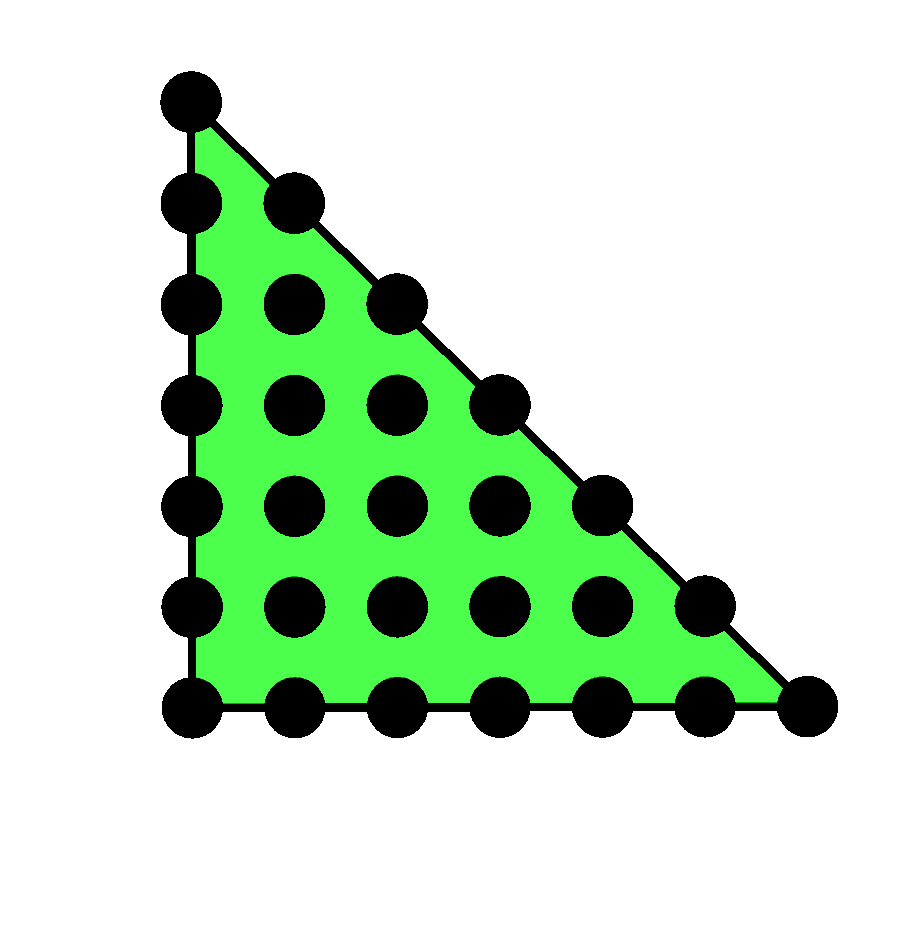
\includegraphics[width=\threefigsfull]{chapters/kirby-6/png/CG6_2d.png}}
\end{figure}


\begin{figure}
  \ffigbox{\caption{The Lagrange $\mathrm{CG}_{q}$ tetrahedron for $q = 1,2,3,4,5,6$.}
           \label{kirby-6:fig:lagrange:3d}}
  {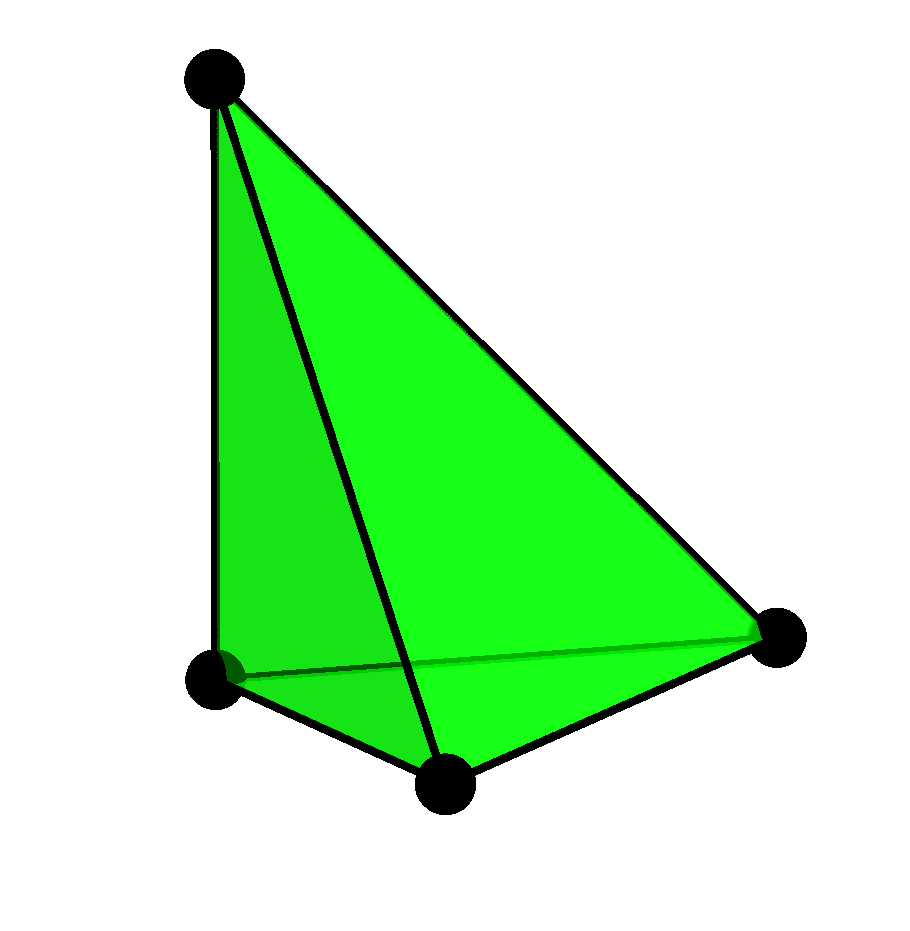
\includegraphics[width=\threefigsfull]{chapters/kirby-6/png/CG1_3d.png}
   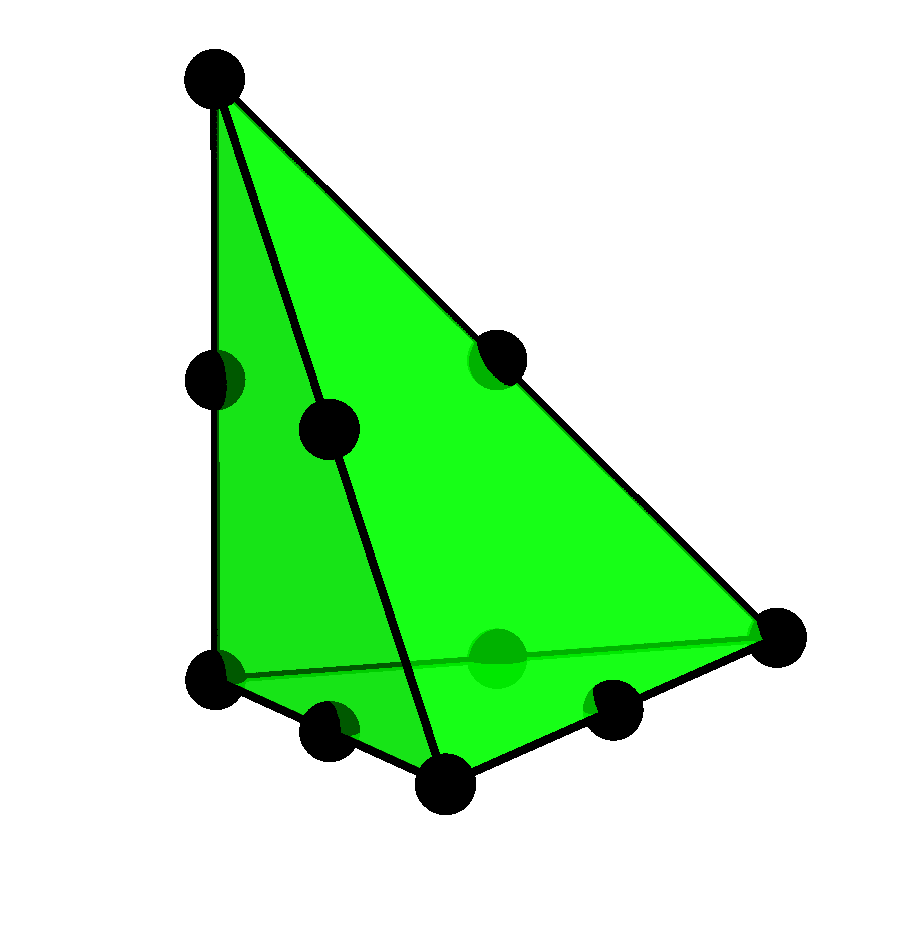
\includegraphics[width=\threefigsfull]{chapters/kirby-6/png/CG2_3d.png}
   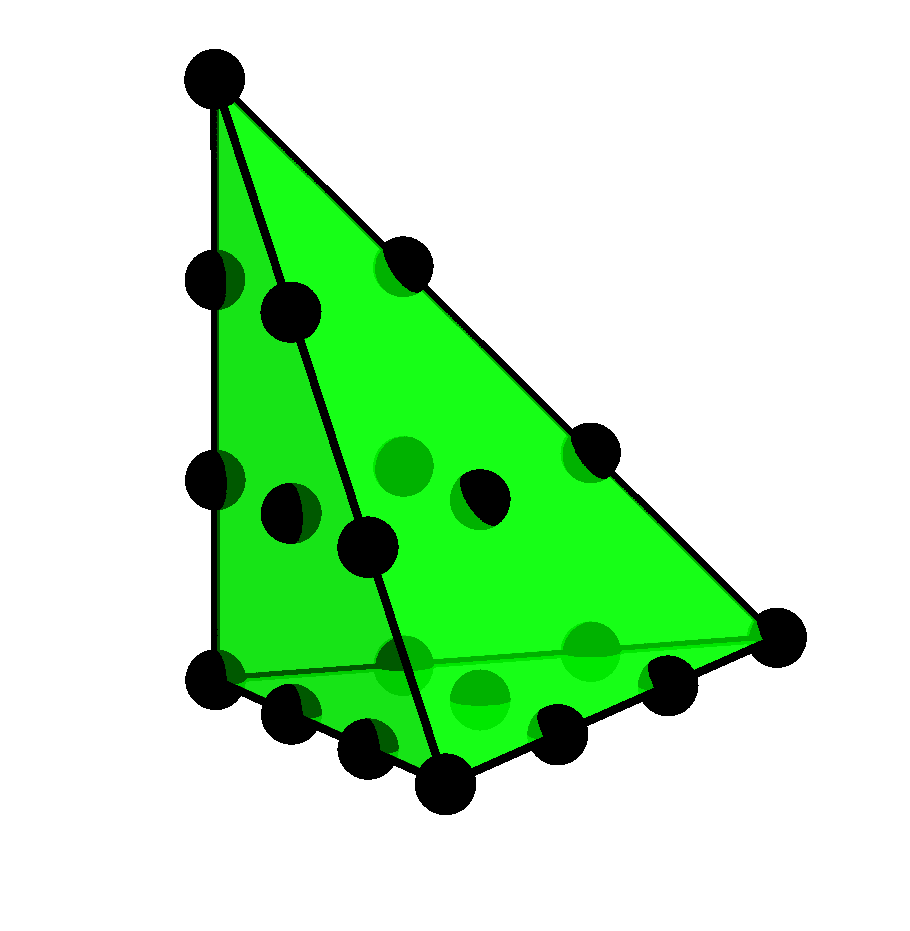
\includegraphics[width=\threefigsfull]{chapters/kirby-6/png/CG3_3d.png} \\
   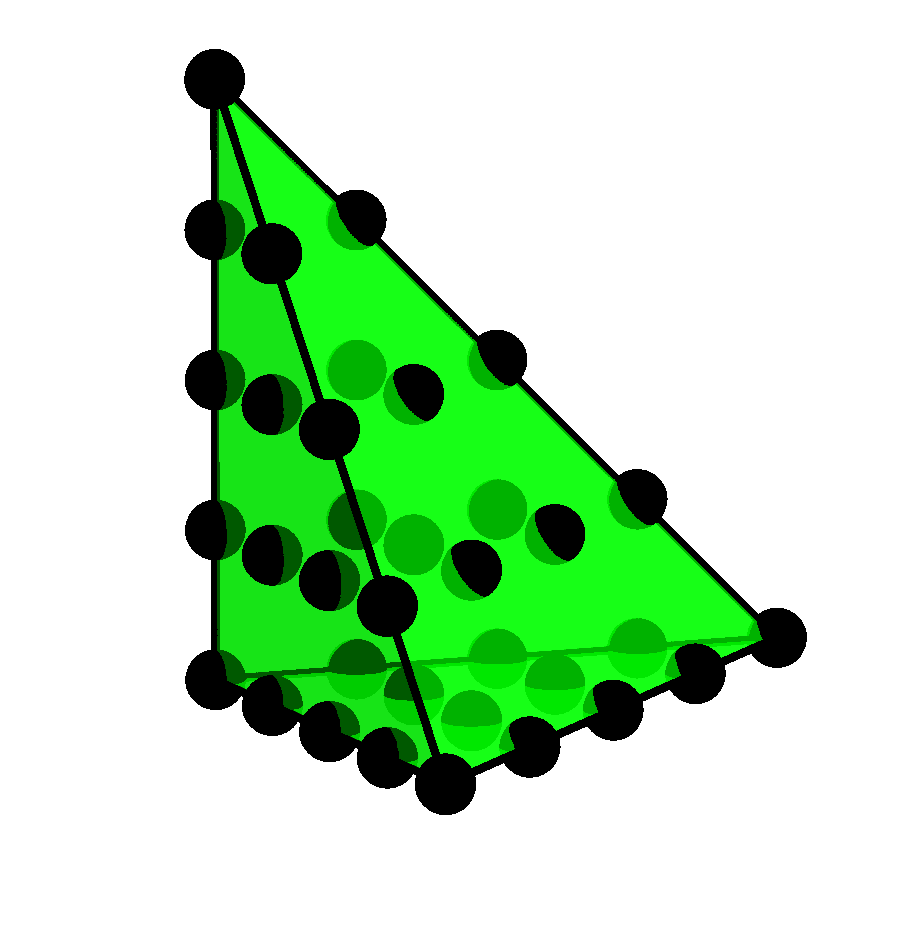
\includegraphics[width=\threefigsfull]{chapters/kirby-6/png/CG4_3d.png}
   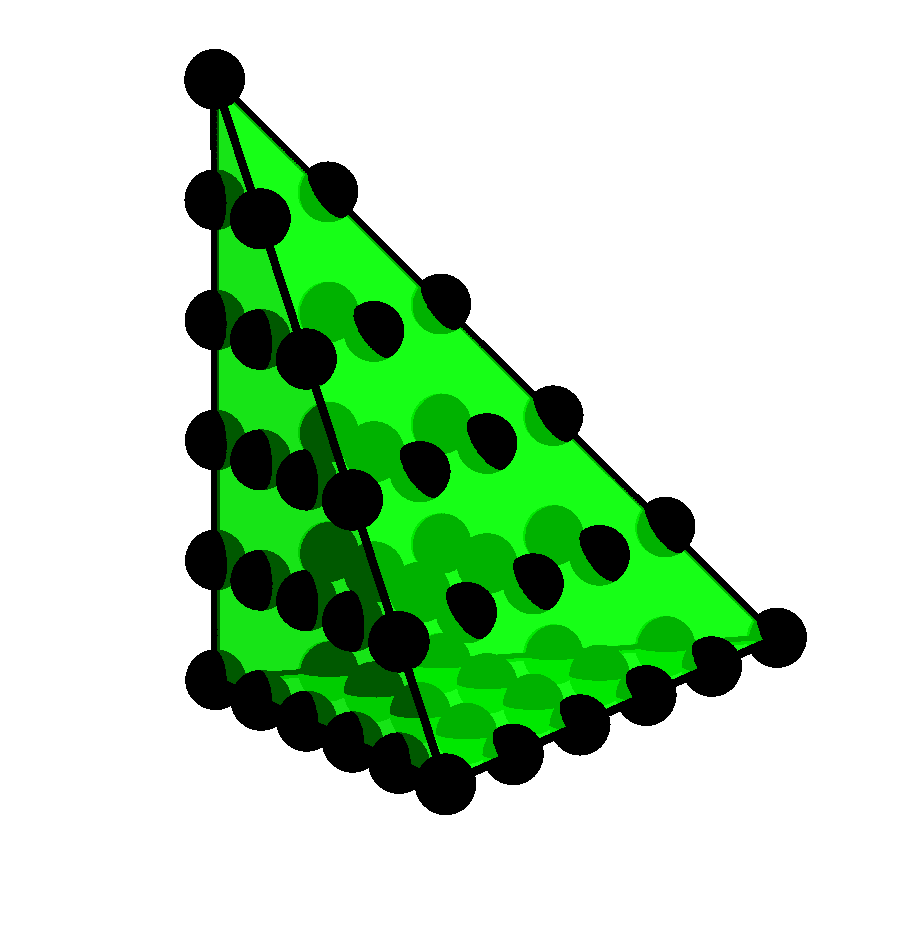
\includegraphics[width=\threefigsfull]{chapters/kirby-6/png/CG5_3d.png}
   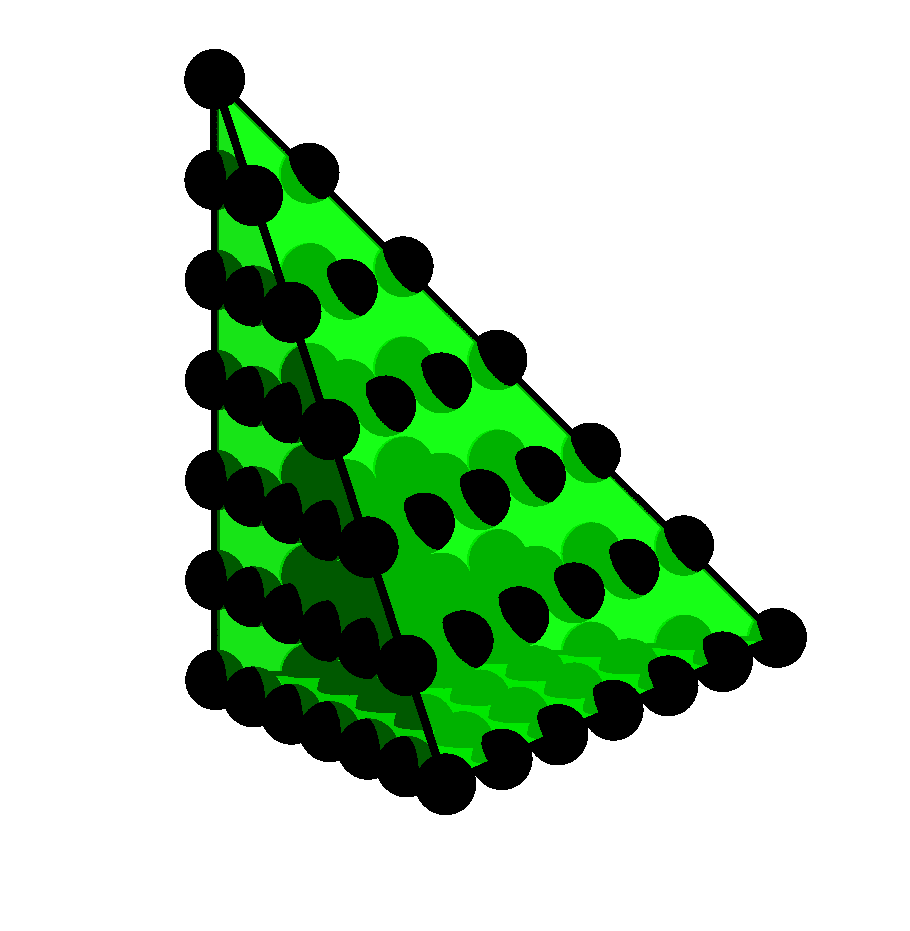
\includegraphics[width=\threefigsfull]{chapters/kirby-6/png/CG6_3d.png}}
\end{figure}




\noindent polynomials, as for the linear Lagrange element. However, in contrast to
the Lagrange element, the global basis functions are not required to be
continuous at all points; continuity is only imposed at the midpoint of
facets. The element is hence not $H^1$-conforming, but it is typically
used for nonconforming approximations of $H^1$ functions (and vector
fields). Other applications of the Crouzeix--Raviart element includes
linear elasticity \citep{HansboLarson2003} and Reissner--Mindlin plates
\citep{ArnoldFalk1989}.

\begin{figure}
  \centering
  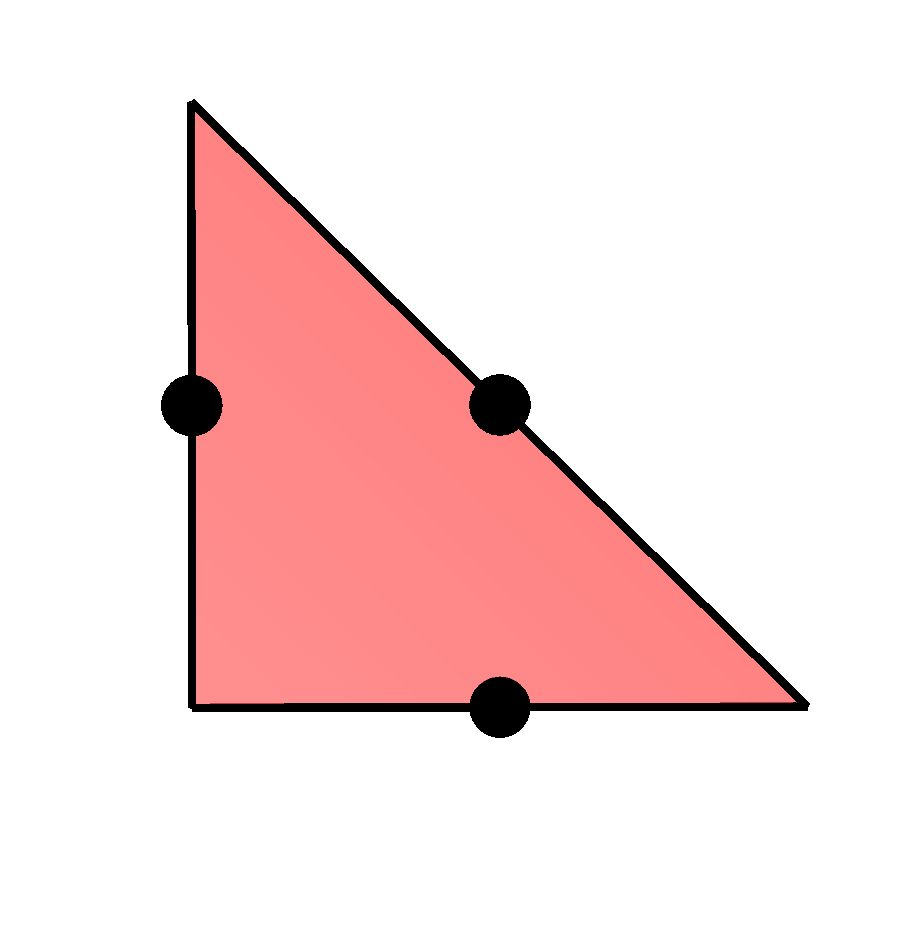
\includegraphics[width=\twofigs]{chapters/kirby-6/png/CR1_2d.png}
  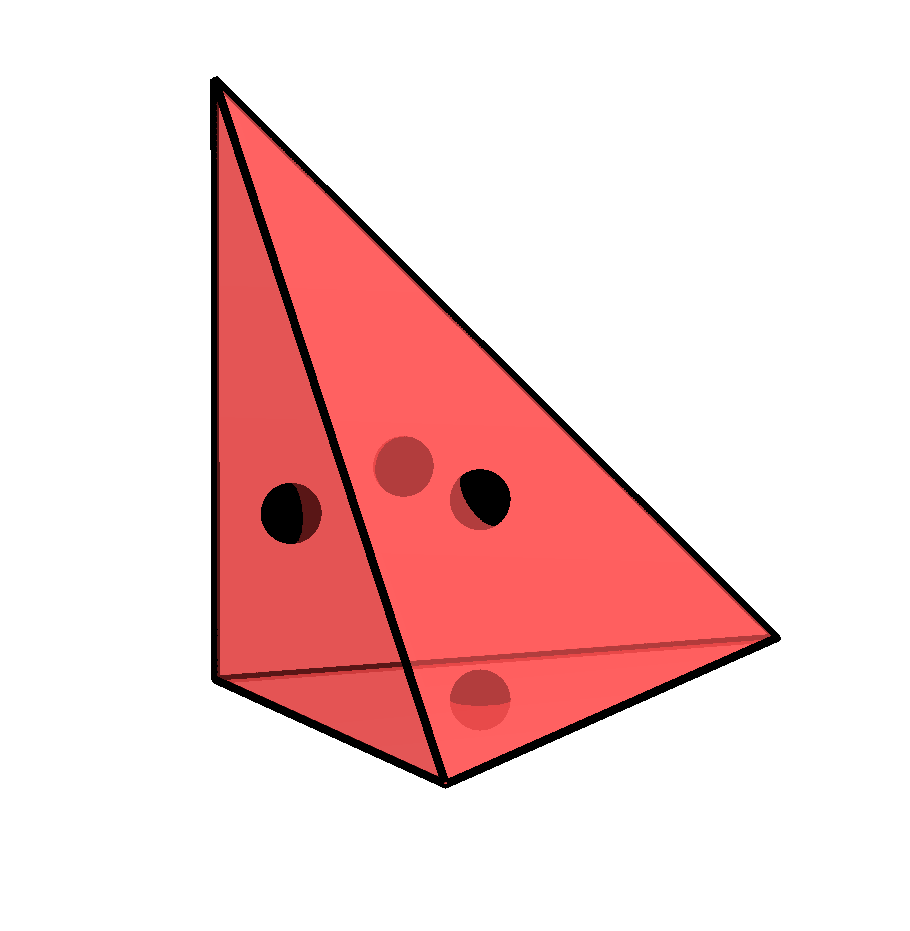
\includegraphics[width=\twofigs]{chapters/kirby-6/png/CR1_3d.png}
  \caption{Illustration of the Crouzeix--Raviart elements on
    triangles and tetrahedra. The degrees of freedom are point
    evaluation at the midpoint of each facet.}
  \label{kirby-6:fig:cr:tri}
\end{figure}

\begin{definition}[Crouzeix--Raviart element]
  The (linear) Crouzeix--Raviart element ($\mathrm{CR}$) is defined by
  \begin{align}
    T &\in \{ \mathrm{triangle}{}, \mathrm{tetrahedron}{}\}, \\
    \CiarletSpace &= \Poly{1}(T), \\
    \ell_i(v) &= v(x^i), \quad i = 1, \dots, n.
  \end{align}
  where $\{x^i\}$ are the barycenters (midpoints) of each facet of the
  domain $T$.
\end{definition}
The dimension of the Crouzeix--Raviart element on $T \subset \R^d$ is
thus
\begin{equation}
  n = d + 1
\end{equation}
for $d = 2, 3$.


Letting $\Pi_T$ denote the interpolation operator defined by the
degrees of freedom, the Crouzeix--Raviart element interpolates as the
linear Lagrange element \citep[Chapter 3.I]{Braess2007}:
\begin{equation}
  ||u - \Pi_T u||_{H^1(T)} \leqslant C \, h_T |u|_{H^2(T)}, \quad
  ||u - \Pi_T u||_{L^2(T)} \leqslant C \, h_T^{2} |u|_{H^2(T)}.
\end{equation}
Vector-valued Crouzeix--Raviart elements can be defined by using a
Crouzeix--Raviart element for each component, or by using facet normal
and facet tangential components at the midpoints of each facet as
degrees of freedom. The Crouzeix--Raviart element can be extended to
higher odd degrees ($q=3,5,7\,\ldots$) \citep{CrouzeixFalk1989}.

%------------------------------------------------------------------------------
\section{$\Hdiv$ finite elements}

The Sobolev space $\Hdiv$ consists of vector fields for which the
components and the weak divergence are square-integrable. This is a
weaker requirement than for a $d$-vector field to be in $[H^1]^d$ (for
$d \geqslant 2$). This space naturally occurs in connection with mixed
formulations of second-order elliptic problems, porous media flow, and
elasticity equations. For a finite element family to be
$\Hdiv$-conforming, each component need not be continuous, but the
normal component must be continuous. In order to ensure such
continuity, the degrees of freedom of $\Hdiv$-conforming elements
usually include normal components on element facets.

The two main families of $\Hdiv$-conforming elements are the
Raviart--Thomas and Brezzi--\break Douglas--Marini elements. These two
families are described below. In addition, the Arnold--Winther element
discretizing the space of symmetric tensor fields with
square-integrable row-wise divergence and the Mardal--Tai--Winther
element are included.


\vspace*{-6pt}\subsection{The Raviart--Thomas element}
\label{sec:raviartthomas}

The Raviart--Thomas element was introduced
by \citet{RaviartThomas1977}. It was the first element to discretize
the mixed form of second-order elliptic equations on triangles. Its
element space $\CiarletSpace$ is designed so that it is the smallest
polynomial space $\CiarletSpace \subset \Poly{q}(T)$, for $q = 1, 2,
\dots$, from which the divergence maps onto $\Poly{q-1}(T)$. Shortly
thereafter, it was extended to tetrahedra and boxes
by \citet{Nedelec1980}. It is therefore sometimes referred to as the
Raviart--Thomas--\nedelec{} element. Here, we label both the two- and
three-dimensional versions as the Raviart--Thomas element.

The definition given below is based on the one presented
by \citet{Nedelec1980} (and \citet{BrezziFortin1991}). The original
Raviart--Thomas paper used a slightly different form. Moreover,
Raviart and Thomas originally started counting at $q = 0$. Hence, the
lowest degree element is traditionally called the $\mathrm{RT}_0$
element.  For the sake of consistency, such that a finite element of
polynomial degree $q$ is included in $\Poly{q}(T)$, we here label the
lowest degree elements by $q = 1$ instead (as did also \nedelec{}).

\begin{definition}[Raviart--Thomas element]
  The Raviart--Thomas element ($\mathrm{RT}_q$) is
  defined for $q = 1, 2, \dots$ by
  \begin{align}
    T &\in \{ \mathrm{triangle}{}, \mathrm{tetrahedron}{}\}, \\
    \CiarletSpace &= [\Poly{q-1}(T)]^d  + x \Poly{q-1}(T), \\
    \mathcal{L} &=
    \left \{
    \begin{array}{ll}
      \int_{f} v \cdot n \, p \ds,
      & \text{ for a set of basis functions } p \in \Poly{q-1}(f)
      \text{ for each facet } $f$, \\
      \int_{T} v \cdot p \dx,
      & \text{ for a set of basis functions } p \in [\Poly{q-2}(T)]^d
      \text{ for } q \geqslant 2. \\
    \end{array}
    \right .
  \end{align}
\end{definition}

\begin{figure}
  \centering
  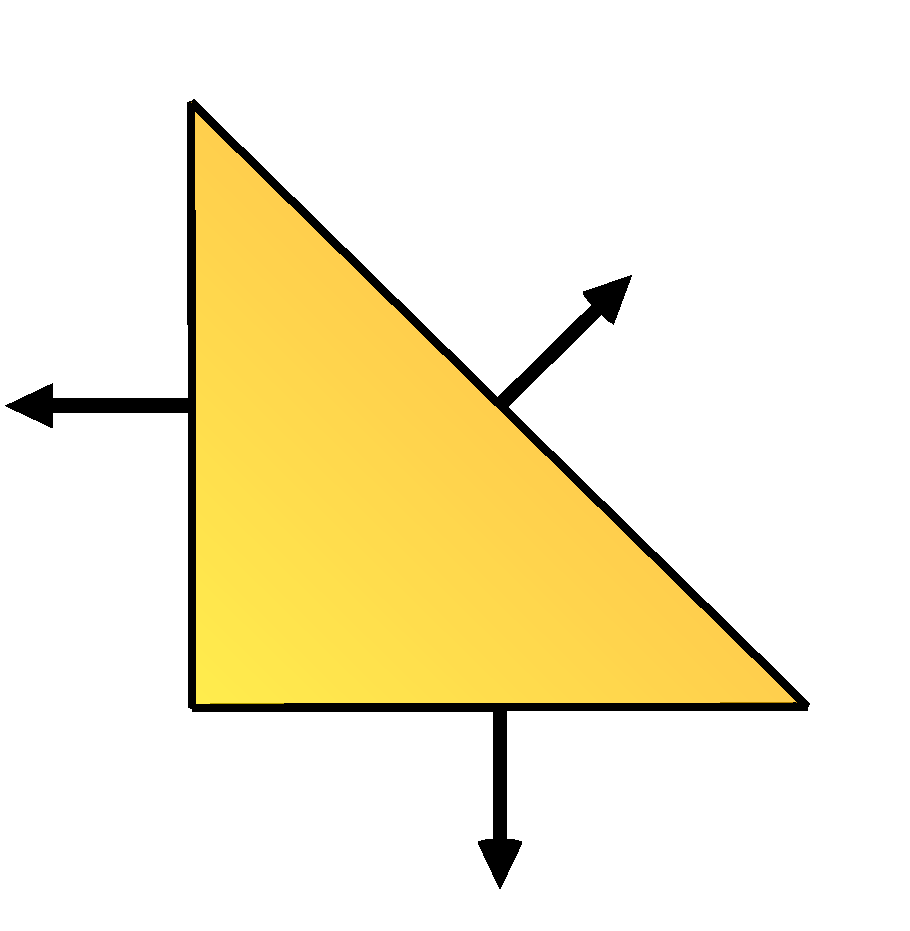
\includegraphics[width=\threefigs]{chapters/kirby-6/png/RT1_2d.png}
  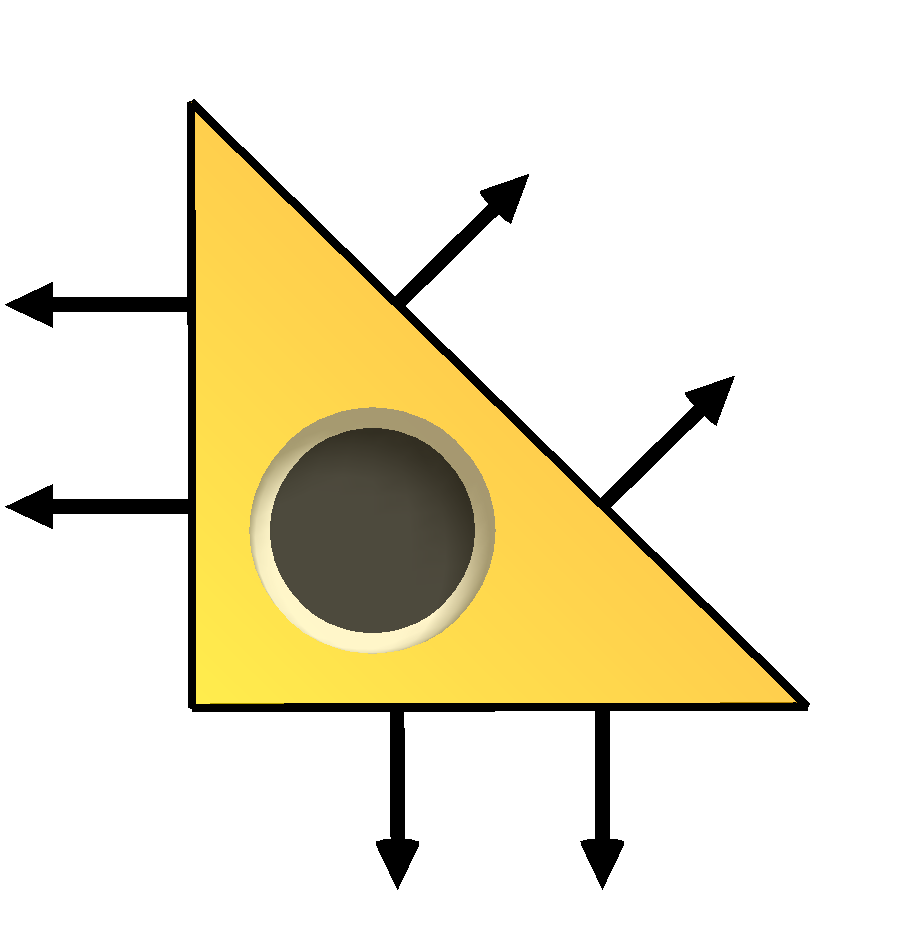
\includegraphics[width=\threefigs]{chapters/kirby-6/png/RT2_2d.png}
  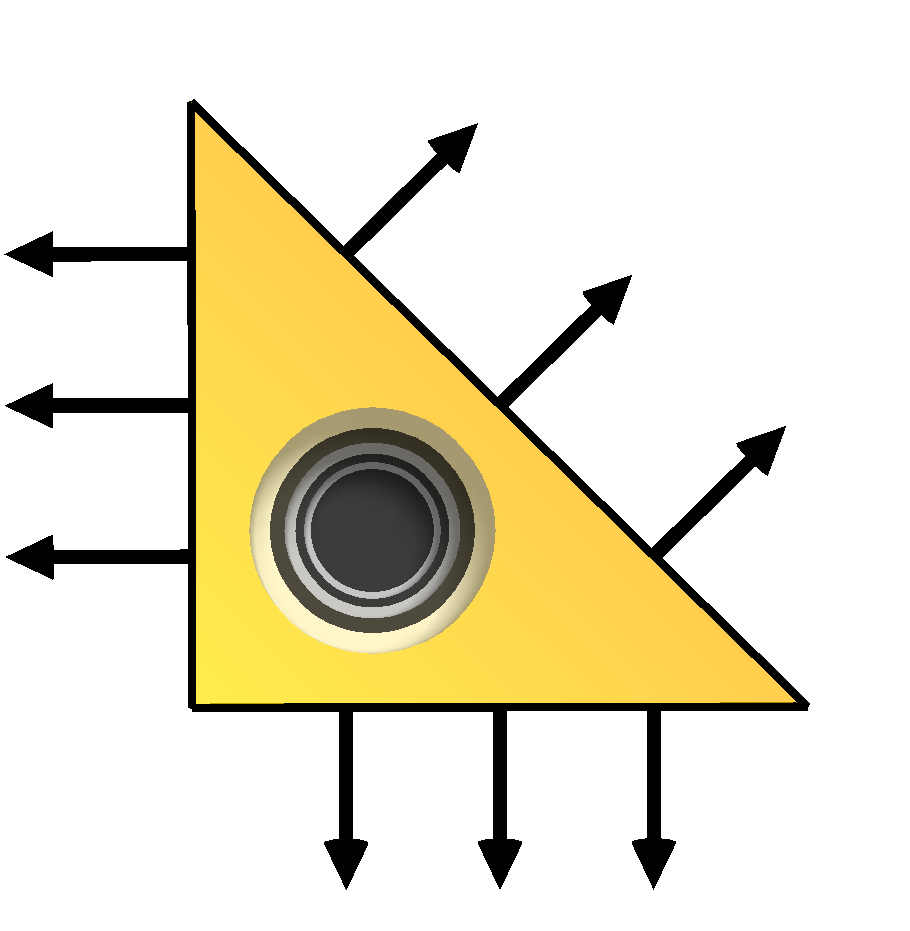
\includegraphics[width=\threefigs]{chapters/kirby-6/png/RT3_2d.png} \\
  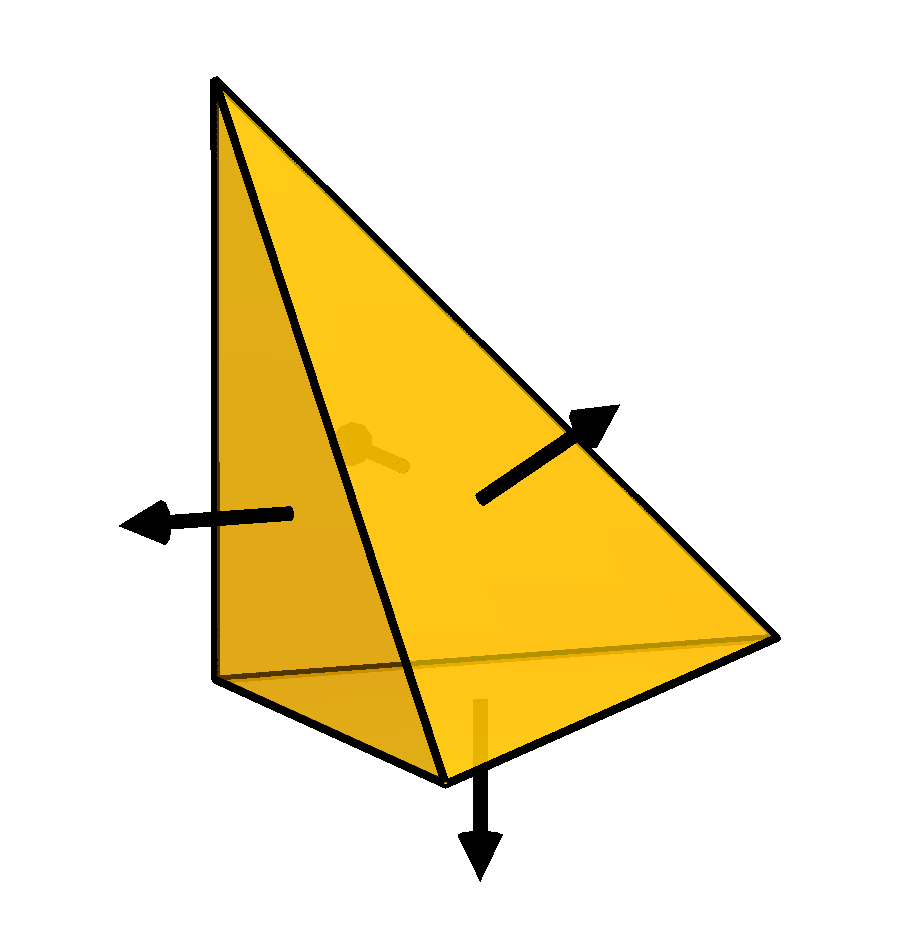
\includegraphics[width=\threefigs]{chapters/kirby-6/png/RT1_3d.png}
  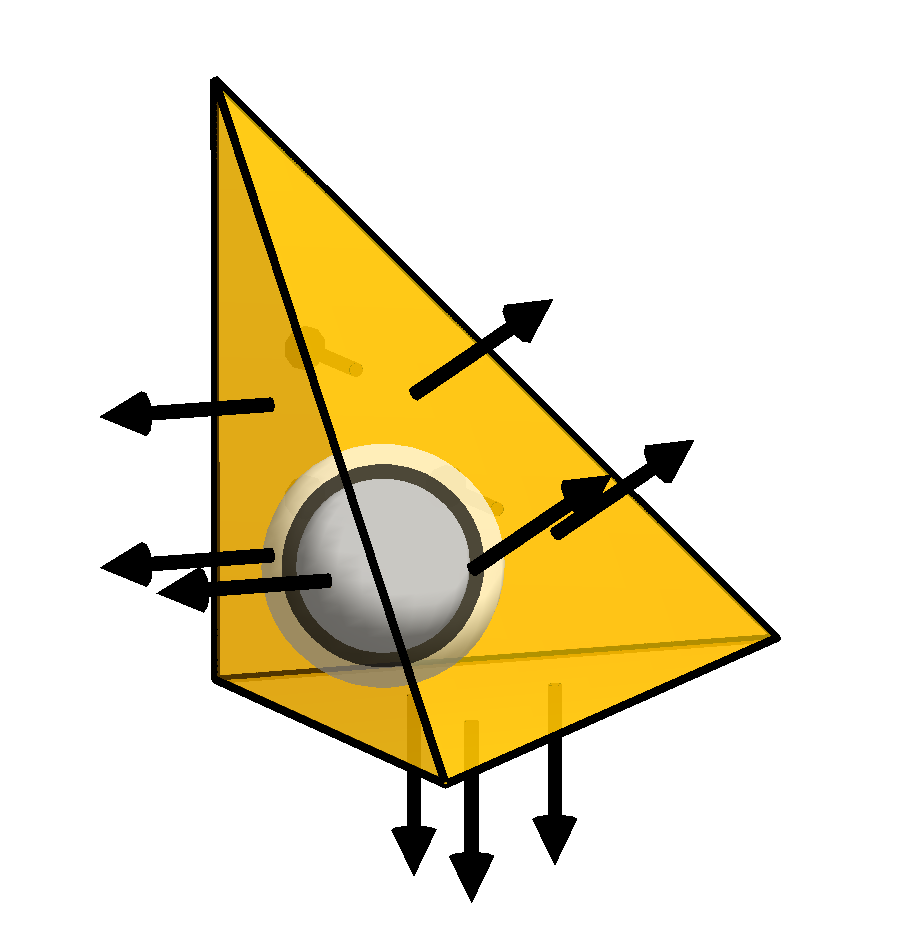
\includegraphics[width=\threefigs]{chapters/kirby-6/png/RT2_3d.png}
  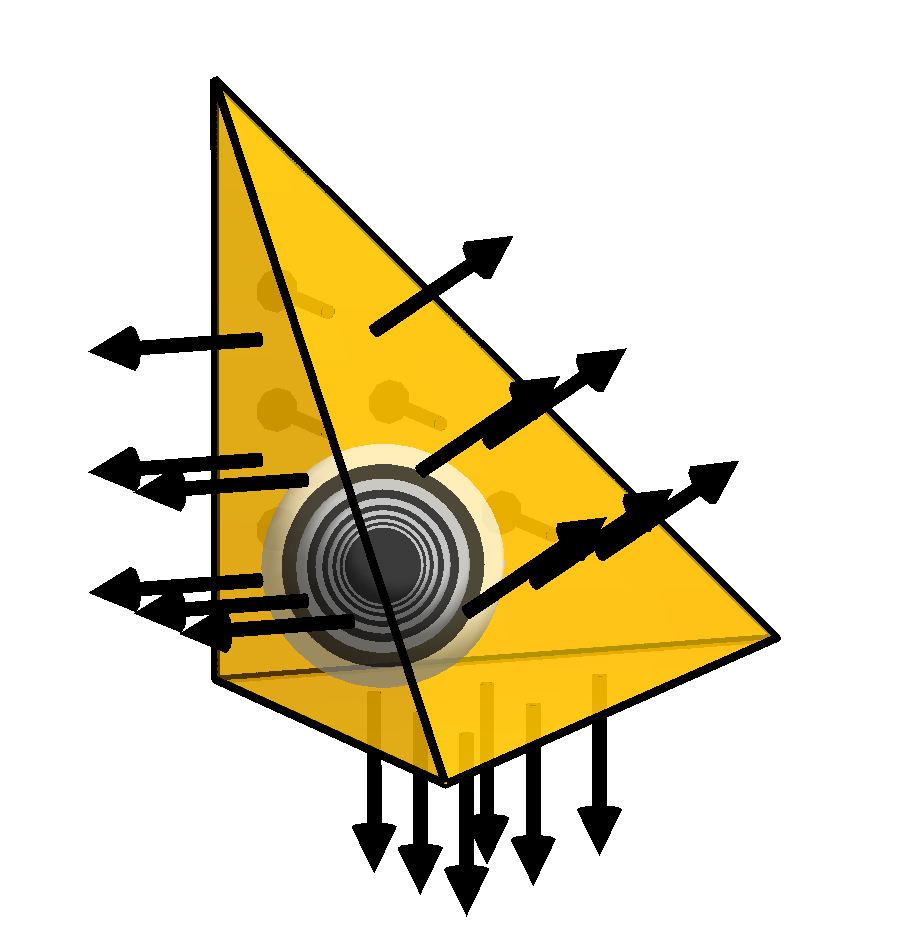
\includegraphics[width=\threefigs]{chapters/kirby-6/png/RT3_3d.png}
  \caption{Illustration of the degrees of freedom for the first,
    second and third degree Raviart--Thomas elements on triangles
    and tetrahedra. The degrees of freedom are moments of the normal
    component against $\Poly{q-1}$ on facets (edges and faces,
    respectively) and, for the higher degree elements, interior
    \hbox{moments} against $[\Poly{q-2}]^d$. Alternatively, as indicated in
    this \hbox{illustration}, the moments of normal \hbox{components} may be
    replaced by point evaluation of normal components.}
  \label{kirby-6:fig:rt}
\vspace*{-12pt}
\end{figure}

As an example, the lowest degree Raviart--Thomas space on triangles is a
three-dimensional space and consists of vector fields of the form
\begin{equation}
  v(x) = \alpha + \beta x,
\end{equation}
where $\alpha$ is a vector-valued constant, and $\beta$ is a scalar
constant.

The dimension of $\mathrm{RT}_q$ is
\begin{equation}
  n(q) = \left \{
  \begin{array}{ll}
  q (q + 2), & T \text{ triangle}, \\
  \frac{1}{2} q (q + 1)(q + 3), & T \text{ tetrahedron}.\\
  \end{array}
  \right .
\end{equation}
Letting $\Pi_T^q$ denote the interpolation operator defined by the
degrees of freedom above for $q = 1, 2, \dots$, we have
that \citep[Chapter III.3]{BrezziFortin1991}
\begin{equation}
  ||u - \Pi_T^q u||_{H(\mathrm{div})(T)} \leqslant C \, h_T^{q} |u|_{H^{q+1}(T)}, \quad
  ||u - \Pi_T^q u||_{L^2(T)} \leqslant C \, h_T^{q} |u|_{H^{q}(T)}.
\end{equation}

\begin{figure}[t!]
  \centering
 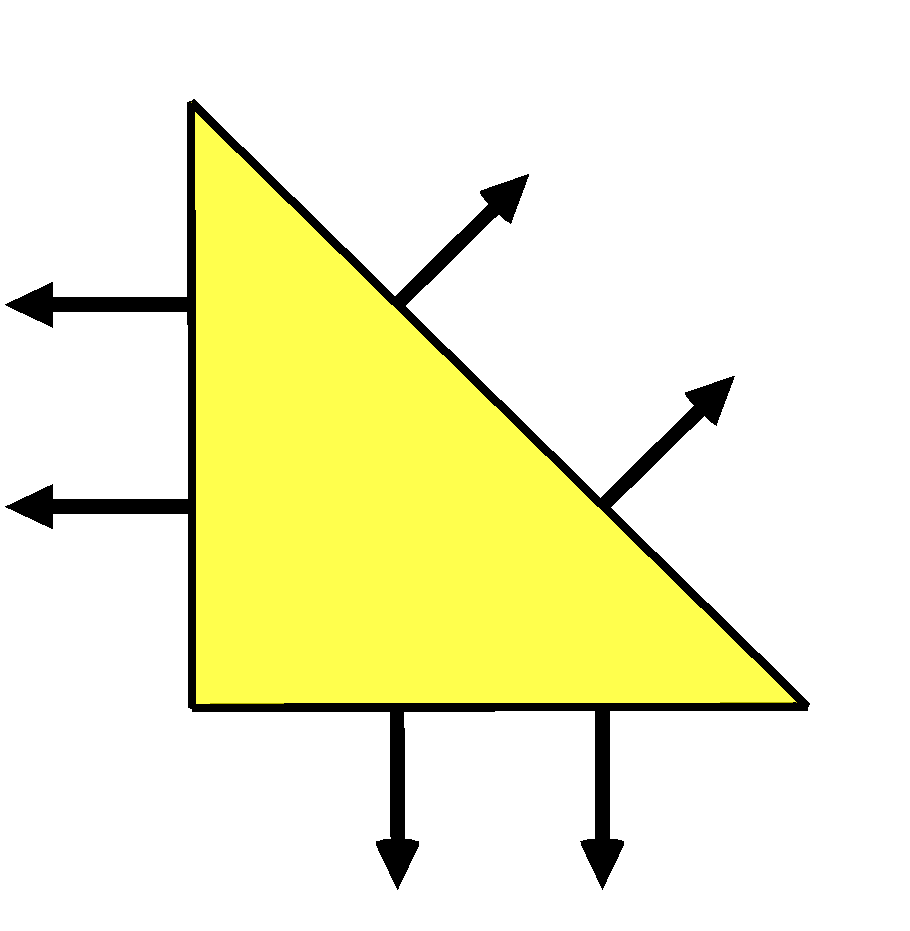
\includegraphics[width=\threefigs]{chapters/kirby-6/png/BDM1_2d.png}
  \includegraphics[width=\threefigs]{chapters/kirby-6/png/BDM2_2d.png}
  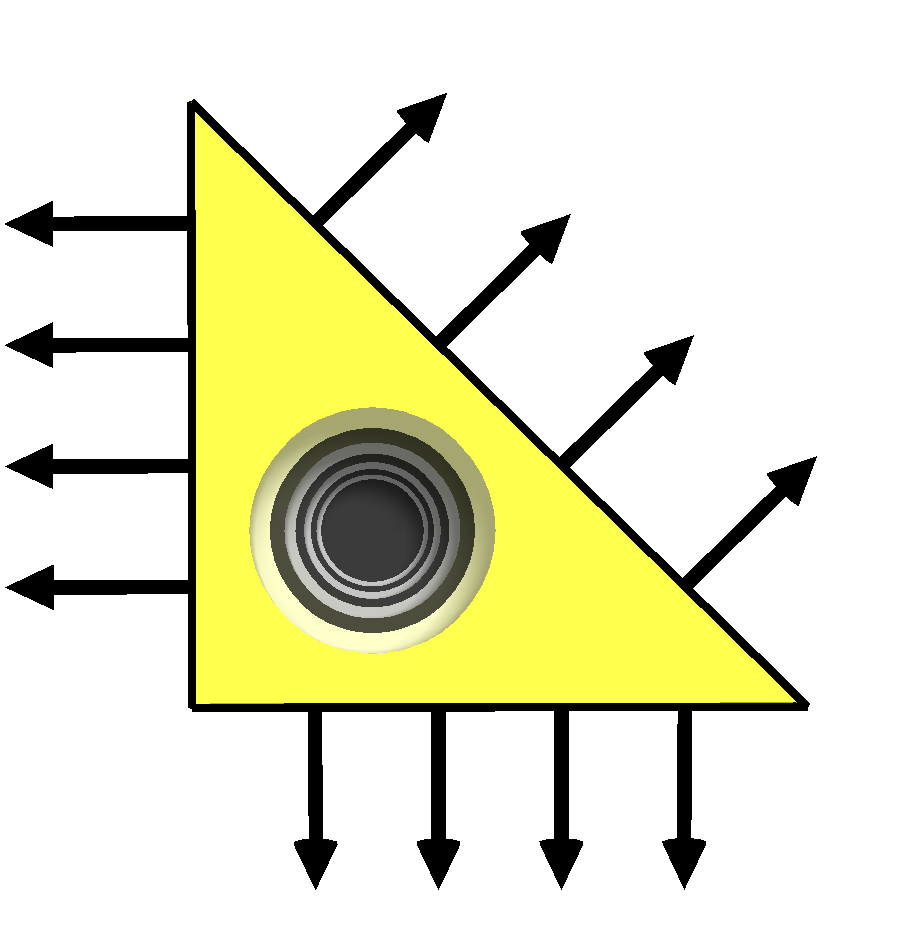
\includegraphics[width=\threefigs]{chapters/kirby-6/png/BDM3_2d.png} \\
  \includegraphics[width=\threefigs]{chapters/kirby-6/png/BDM1_3d.png}
  \includegraphics[width=\threefigs]{chapters/kirby-6/png/BDM2_3d.png}
  \includegraphics[width=\threefigs]{chapters/kirby-6/png/BDM3_3d.png}
  \caption{Illustration of the first, second and third degree
    Brezzi--Douglas--Marini elements on triangles and tetrahedra.
    The degrees of freedom are moments of the normal component
    against $\Poly{q}$ on facets (edges and faces, respectively)
    and, for the higher degree elements, interior moments against
    $\mathrm{NED}^1_{q-1}$. Alternatively, as indicated in this
    illustration, the moments of normal components may be replaced
    by point evaluation of normal components.}
  \label{kirby-6:fig:bdm}
%% 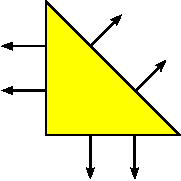
\includegraphics[width=\threefigs]{kirby-6/BDM1_2d}
%%  \includegraphics[width=\threefigs]{kirby-6/BDM2_2d}
%%  \includegraphics[width=\threefigs]{kirby-6/BDM3_2d} \\
%%  \includegraphics[width=\threefigs]{kirby-6/BDM1_3d}
%%  \includegraphics[width=\threefigs]{kirby-6/BDM2_3d}
%%  \includegraphics[width=\threefigs]{kirby-6/BDM3_3d}
\end{figure}


%------------------------------------------------------------------------------
\subsection{The Brezzi--Douglas--Marini element}

The Brezzi--Douglas--Marini element was introduced by Brezzi,
Douglas and Marini in two dimensions (for triangles) in
\citet{BrezziDouglasMarini1985}. The element can be viewed as
an alternative to the Raviart--Thomas element using a complete
polynomial space. It was later extended to three dimensions
(tetrahedra, prisms and cubes) in \citet{Nedelec1986} and
\citet{BrezziDouglasDuranFortin1987}. The definition given here is based
on that of \citet{Nedelec1986}.

The Brezzi--Douglas--Marini element was introduced for mixed
formulations of second-order elliptic equations. However, it is also
useful for weakly symmetric discretizations of the elastic stress
tensor; see \citet{FarhloulFortin1997, ArnoldFalkWinther2007}.

\begin{definition}[Brezzi--Douglas--Marini element]
  The Brezzi--Douglas--Marini element ($\mathrm{BDM}_q$)
  is\break \hbox{defined} for $q = 1, 2, \dots$ by
  \begin{align}
    T &\in \{ \mathrm{triangle}{}, \mathrm{tetrahedron}{}\}, \\
    \CiarletSpace &= [\Poly{q}(T)]^d, \\
    \mathcal{L} &=
    \left \{
    \begin{array}{ll}
      \int_{f} v \cdot n p \ds,
      & \text{ for a set of basis functions } p \in \Poly{q}(f)
      \text{ for each facet } $f$, \\
      \int_{T} v \cdot p \dx, &
      \text{ for a set of basis functions } p \in \mathrm{NED}^1_{q-1}(T)
      \text{ for } q \geqslant 2. \\
    \end{array}
    \right.
  \end{align}
  where $\mathrm{NED}^1$ refers to the \nedelec{} $\Hcurl$ elements of
  the first kind, defined below in Section~\ref{sec:nedelec:first}.
\end{definition}


The dimension of $\mathrm{BDM}_q$ is
\begin{equation}
  n(q) = \left \{
    \begin{array}{ll}
      (q + 1)(q + 2), & T \text{ triangle},  \\
      \frac{1}{2} (q + 1)(q + 2)(q + 3), & T \text{ tetrahedron}.\\
    \end{array}
    \right .
\end{equation}
Letting $\Pi_T^q$ denote the interpolation operator defined by the
degrees of freedom for $q = 1, 2, \dots$, we have that \citep[Chapter
  III.3]{BrezziFortin1991}
\begin{equation}
  ||u - \Pi_T^q u||_{H(\mathrm{div})(T)} \leqslant C \, h_T^{q} |u|_{H^{q+1}(T)}, \quad
  ||u - \Pi_T^q u||_{L^2(T)} \leqslant C \, h_T^{q+1} |u|_{H^{q+1}(T)}.
\end{equation}

A slight modification of the Brezzi--Douglas--Marini element
constrains the element space $\CiarletSpace$ by only allowing normal
components on the boundary of polynomial degree $q - 1$ (rather than
the full polynomial degree~$q$). Such an element was suggested on
rectangles by \citet{BrezziDouglasFortinEtAl1987}, and the triangular
analogue was given in \citet{BrezziFortin1991}. In similar spirit,
elements with differing degrees on the boundary suitable for varying
the polynomial degree between triangles were derived
in \citet{BrezziDouglasMarini1985a}.

\subsection{The Mardal-Tai-Winther element}

The Mardal--Tai--Winther element was introduced
in \citet{MardalTaiWinther2002} as a finite element suitable for the
velocity space for both Darcy and Stokes flow in two dimensions. In
the Darcy flow equations, the velocity space only requires
$\Hdiv$-regularity. Moreover, discretizations based on
$H^1$-conforming finite elements are typically not stable. On the
other hand, for the Stokes equations, the velocity space does
stipulate $H^1$-regularity. The Mardal--Tai--Winther element is
$\Hdiv$-conforming, but\break $H^1$-nonconforming. The element was extended
to three dimensions in \citet{TaiWinther2006}, but we only present the
two-dimensional case here.

\begin{definition}[Mardal--Tai--Winther element]
  The Mardal--Tai--Winther element ($\mathrm{MTW}$) is defined by
  \begin{align}
    T &= \mathrm{triangle}{},  \\
    \CiarletSpace &= \{ v \in [\Poly{3}(T)]^2,
                     \text{ such that } \Div v \in \Poly{0}(T)
                     \text{ and } v \cdot n|_{f} \in \Poly{1}(T)
                     \text{ for each facet } f \}, \\
    \mathcal{L} &=
    \left \{
    \begin{array}{ll}
      \int_{f} v \cdot n \, p \ds,
      & \text{ for a set of basis functions } p \in \Poly{1}(f)
      \text{ for each facet } $f$, \\
      \int_{f} v \cdot t \, \ds,
      & \text{ for each facet } $f$. \\
    \end{array}
    \right .
  \end{align}
\end{definition}

\begin{figure}
  \centering
    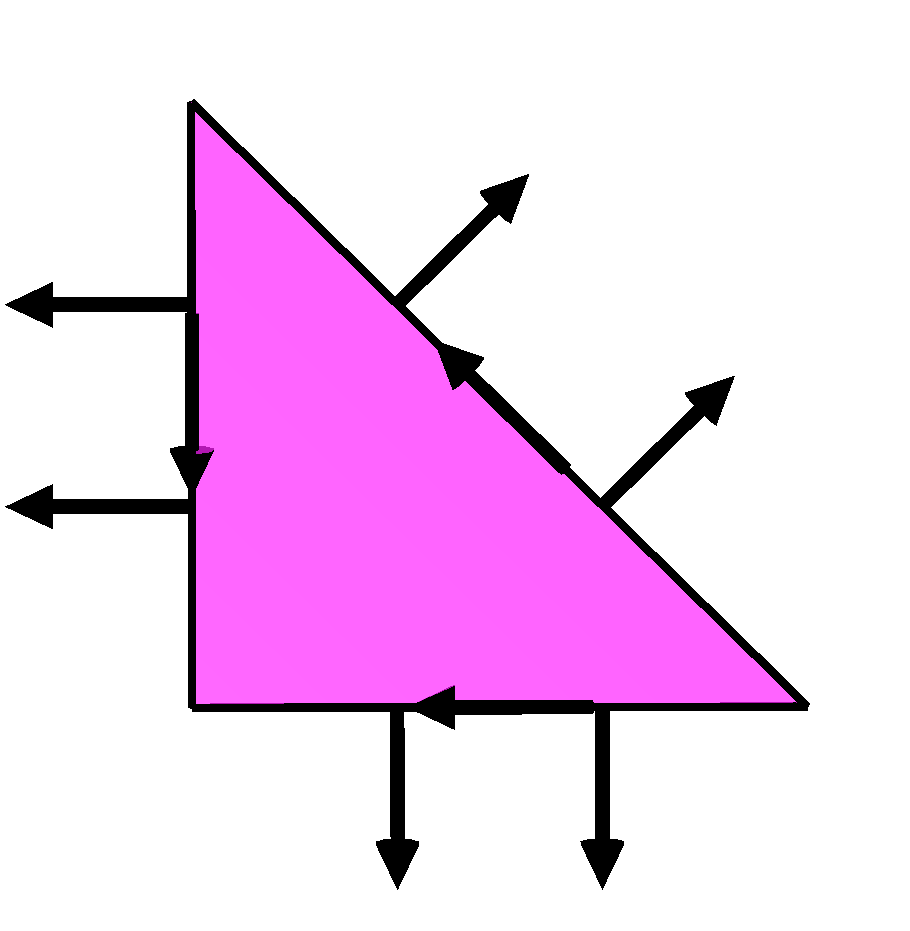
\includegraphics[width=\smallfig]{chapters/kirby-6/png/MTW_2d.png}
  \caption{Illustration of the Mardal--Tai--Winther element. The
    degrees of freedom are two moments of the normal component on
    each facet and one moment of the tangential component on each
    facet. In this figure, the moments of normal components are
    illustrated by point evaluation of normal components.}
\end{figure}
The dimension of $\mathrm{MTW}$ is
\begin{equation}
  n = 9.
\end{equation}
Letting $\Pi_T$ denote the interpolation operator defined by the
degrees of freedom, we have that
\begin{equation}
  ||u - \Pi_T u||_{H^1(T)} \leqslant C \, h_T |u|_{H^2(T)}, \;
  ||u - \Pi_T u||_{H(\mathrm{div})(T)} \leqslant C \, h_T |u|_{H^{2}(T)}, \;
  ||u - \Pi_T u||_{L^2(T)} \leqslant C \, h_T^{2} |u|_{H^2(T)}.
\end{equation}

\subsection{The Arnold--Winther element}

The Arnold--Winther element was introduced
by \citet{ArnoldWinther2002}. This paper presented the first stable
mixed (non-composite) finite element for the stress--displacement
formulation of linear elasticity. The finite element used for the
stress space is what is presented as the Arnold--Winther element
here. This finite element is a symmetric tensor element that is
row-wise $\Hdiv$-conforming. The finite element was introduced for a
hierarchy of polynomial degrees and extended to \hbox{three-dimensions}
in \citet{AdamsCockburn2005} and \citet{ArnoldAwanouWinther2008}, but we
only present the lowest degree two-dimensional case here.

\begin{definition}[Arnold--Winther element]
  The (lowest degree) Arnold--Winther element ($\mathrm{AW}$) is
  defined by
  \begin{align}
    T &= \mathrm{triangle}{},  \\
    \CiarletSpace &= \{ v \in \Poly{3}(T; \mathbb{S}) :
                     \Div v \in \Poly{1}(T; \R^2) \}, \\
    \mathcal{L} &=
    \left \{
    \begin{array}{ll}
      v(x^k)_{ij},  & \text{ for } 1 \leqslant i \leqslant j \leqslant 2
      \text{ at each vertex } x^k \\
      \int_{f} \sum_{j=1}^2 v_{ij} n_j \, p \ds,
      & \text{ for a set of basis functions } p \in \Poly{1}(f),
      \text{ on each facet } $f$, \; 1 \leqslant i \leqslant 2, \\
      \int_{T} v_{ij} \dx,
      & \text{ for } 1 \leqslant i \leqslant j \leqslant 2.
    \end{array}
    \right .
  \end{align}
\end{definition}
The dimension of $\mathrm{AW}$ is
\begin{equation}
  n = 24.
\end{equation}

\begin{figure}
  \centering
  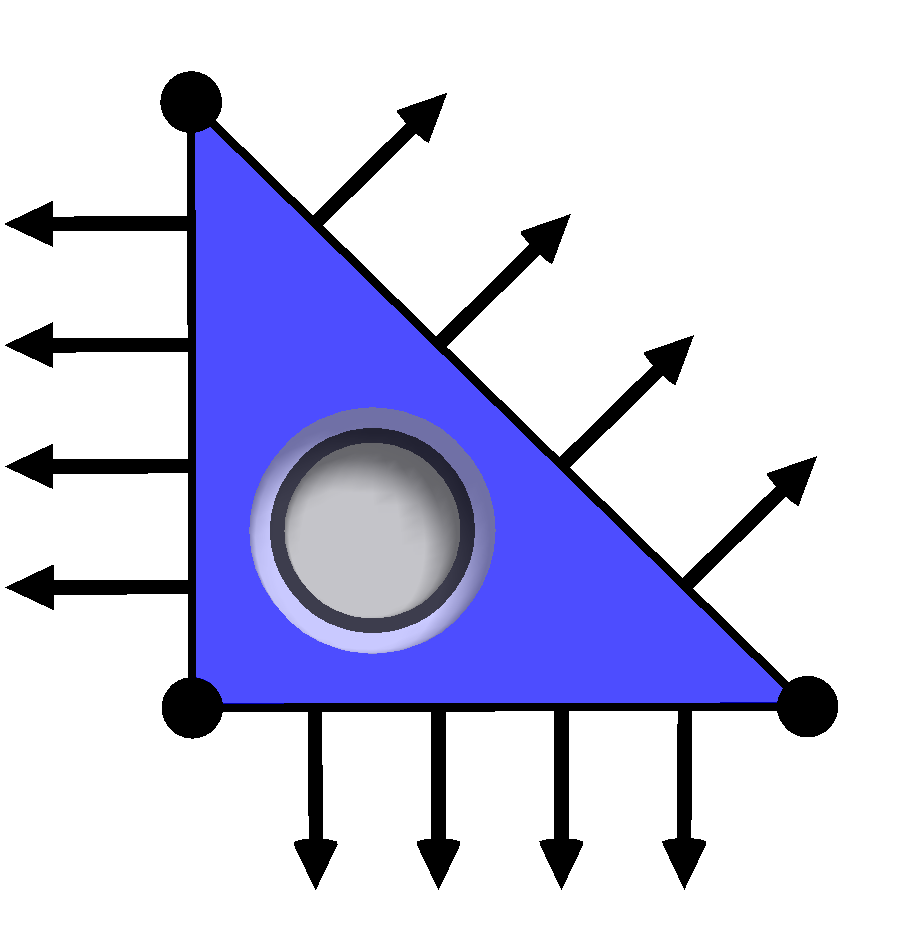
\includegraphics[width=\smallfig]{chapters/kirby-6/png/AW_2d.png}
  \caption{Illustration of the Arnold--Winther element. The
    24 degrees of freedom are point evaluation at the vertices,
    the two first moments of the normal component of each row of
    the tensor field on each facet, and three interior moments.}
\end{figure}

Letting $\Pi_T$ denote the interpolation operator defined by the
degrees of freedom, we have that
\begin{equation}
  ||u - \Pi_T u||_{H(\mathrm{div})(T)} \leqslant C \, h_T^2 |u|_{H^{3}(T)}, \quad
  ||u - \Pi_T u||_{L^2(T)} \leqslant C \, h_T^{3} |u|_{H^3(T)}.
\end{equation}

%------------------------------------------------------------------------------
\section{$\Hcurl$ finite elements}

The Sobolev space $\Hcurl$ arises frequently in problems associated
with electromagnetism. The \nedelec{} elements, also colloquially
referred to as \emph{edge elements}, are much used for such problems,
and stand as a premier example of the power of ``nonstandard''
(meaning not lowest-degree Lagrange) finite elements
\citep{Nedelec1980,Nedelec1986}. For a piecewise polynomial to be
$\Hcurl$-conforming, the tangential component must be
continuous. Therefore, the degrees of freedom for $\Hcurl$-conforming
finite elements typically include tangential components.

There are four families of finite element spaces due to \nedelec,
introduced in the papers \citet{Nedelec1980} and \citet{Nedelec1986}.
The first (1980) paper introduced two families of finite element
spaces on tetrahedra, cubes and prisms: one $\Hdiv$-conforming family
and one $\Hcurl$-conforming family. These families are known as
\nedelec{} $\Hdiv$ elements of the \emph{first kind} and \nedelec{}
$\Hcurl$ elements of the \emph{first kind}, respectively. The $\Hdiv$
elements can be viewed as the three-dimensional extension of the
Raviart--Thomas elements. (These are therefore presented as
Raviart--Thomas elements above.) The first kind \nedelec{} $\Hcurl$
elements are presented below.

The second (1986) paper introduced two more families of finite element
spaces: again, one $\Hdiv$-conforming family and one
$\Hcurl$-conforming family. These families are known as \nedelec{}
$\Hdiv$ elements of the \emph{second kind} and \nedelec{} $\Hcurl$
elements of the \emph{second kind}, respectively. The $\Hdiv$ elements
can be viewed as the three-dimensional extension of the
Brezzi--Douglas--Marini elements. (These are therefore presented as
Brezzi--Douglas--Marini elements above.) The second kind \nedelec{}
$\Hcurl$ elements are presented below.

In his two classic papers, \nedelec{} considered only the
three-dimensional case. However, one can also define a two-dimensional
$\mathrm{curl}$, and two-dimensional $\Hcurl$-conforming finite
element spaces. We present such elements as \nedelec{} elements on
triangles here. Although attributing these elements to \nedelec{} may
be dubious, we include them for the sake of completeness.

In many ways, \nedelec{}'s work anticipates the recently introduced
finite element exterior calculus presented
in \citet{ArnoldFalkWinther2006}, where the first kind spaces appear as
\( \mathcal{P}_q^-\Lambda^k \) spaces and the second kind as \(
\mathcal{P}_q\Lambda^k \). Moreover, the use of a differential
operator (the elastic strain) in \citet{Nedelec1980} to characterize
the function space foreshadows the use of differential complexes
in \citet{ArnoldFalkWinther2006c}.

%------------------------------------------------------------------------------
\subsection{The \nedelec{} $\Hcurl$ element of the first kind}
\label{sec:nedelec:first}

\begin{definition}[\nedelec{} $\Hcurl$ element of the first kind]
  For $q = 1, 2, \dots$, define the space
  \begin{equation}
    S_{q}(T) = \{ s \in [\Poly{q}(T)]^d \, : \, s(x) \cdot x = 0 \quad
    \foralls x \in T\}.
  \end{equation}
  The \nedelec{} element of the first kind ($\mathrm{NED}^1_q$) is
  defined for $q = 1, 2, \dots$ in two dimensions by
  \begin{align}
    T &= \mathrm{triangle}{}, \\
    \CiarletSpace &= [\Poly{q-1}(T)]^2 + S_{q}(T), \\
    \mathcal{L} &=
    \left \{
    \begin{array}{ll}
      \int_{e} v \cdot t \, p \ds,
      &\text{ for a set of basis functions }  p \in \Poly{q-1}(e)
      \text{ for each edge } e, \\
      \int_{T} v \cdot  p \dx,
      &\text{ for a set of basis functions } p \in [\Poly{q-2}(T)]^2,
      \text{ for } q \geqslant 2, \\
    \end{array}
    \right.
  \end{align}
  where $t$ is the edge tangent; and in three dimensions by
  \begin{align}
    T &= \mathrm{tetrahedron}{}, \\
    \CiarletSpace &= [\Poly{q-1}(T)]^3 + S_{q}(T), \\
    \mathcal{L} &=
    \left \{
    \begin{array}{ll}
      \int_{e} v \cdot t \, p \,\mathrm{d}l,
      &\text{ for a set of basis functions } p \in \Poly{q-1}(e)
      \text{ for each edge } e \\
      \int_{f} v \times n \cdot p \ds,
      &\text{ for a set of basis functions } p \in [\Poly{q-2}(f)]^2
      \text{ for each face } f, \text{ for } q \geqslant 2, \\
      \int_{T} v \cdot p \dx,
      &\text{ for a set of basis functions } p \in [\Poly{q-3}]^3,
      \text{ for } q \geqslant 3. \\
    \end{array}
    \right .
  \end{align}
\end{definition}
The dimension of $\mathrm{NED}^1_q$ is
\begin{equation}
  n(q) = \left \{
  \begin{array}{ll}
  q (q + 2), & T \text{ triangle}, \\
  \frac{1}{2} q(q+2)(q+3), & T \text{ tetrahedron}.\\
  \end{array}
  \right .
\end{equation}

\begin{figure}
  \centering
 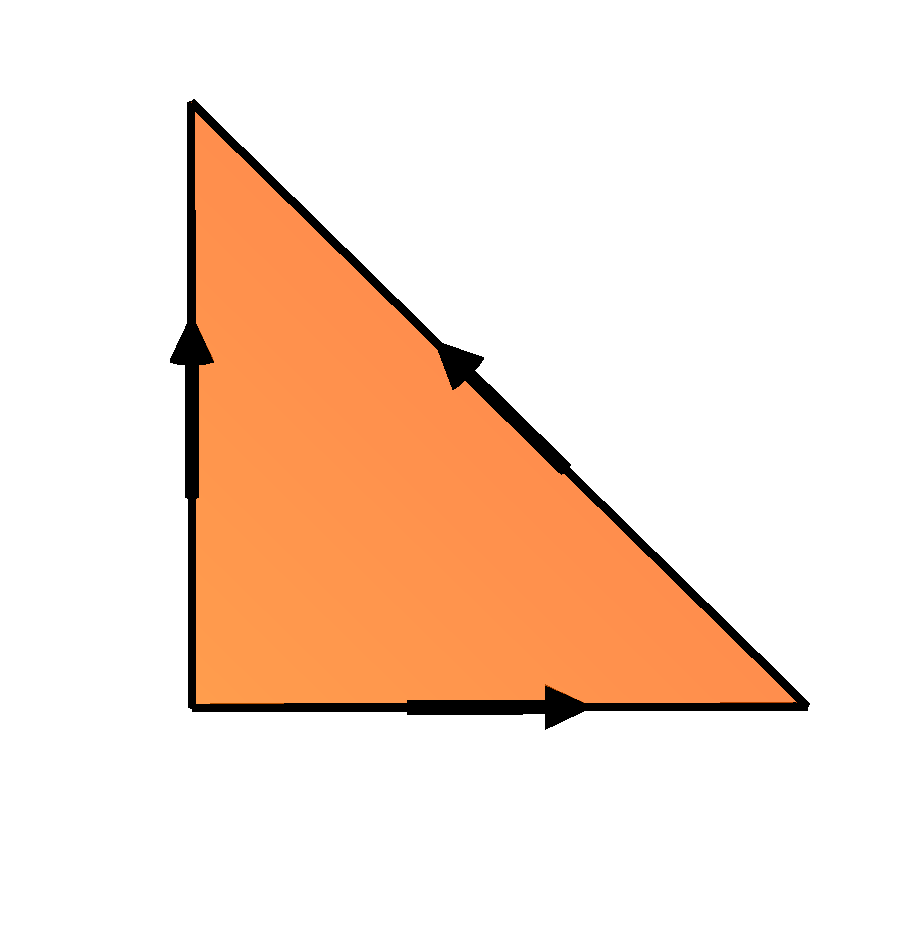
\includegraphics[width=\threefigs]{chapters/kirby-6/png/NED1_1_2d.png}
  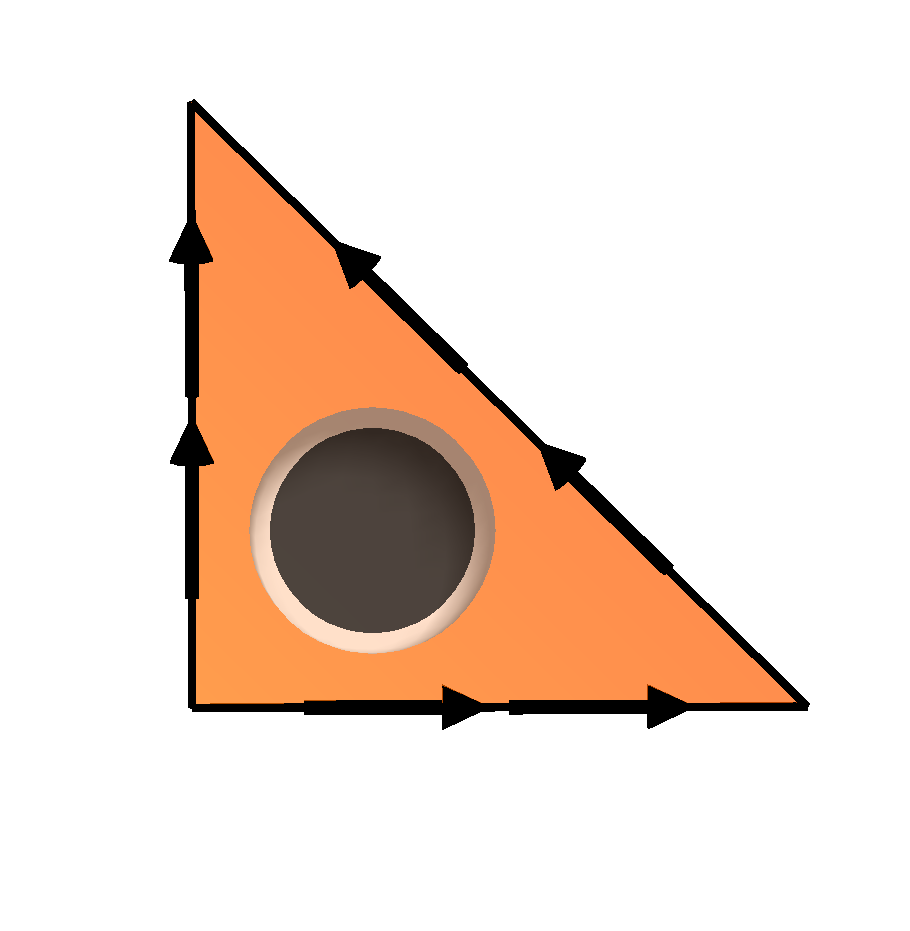
\includegraphics[width=\threefigs]{chapters/kirby-6/png/NED1_2_2d.png}
  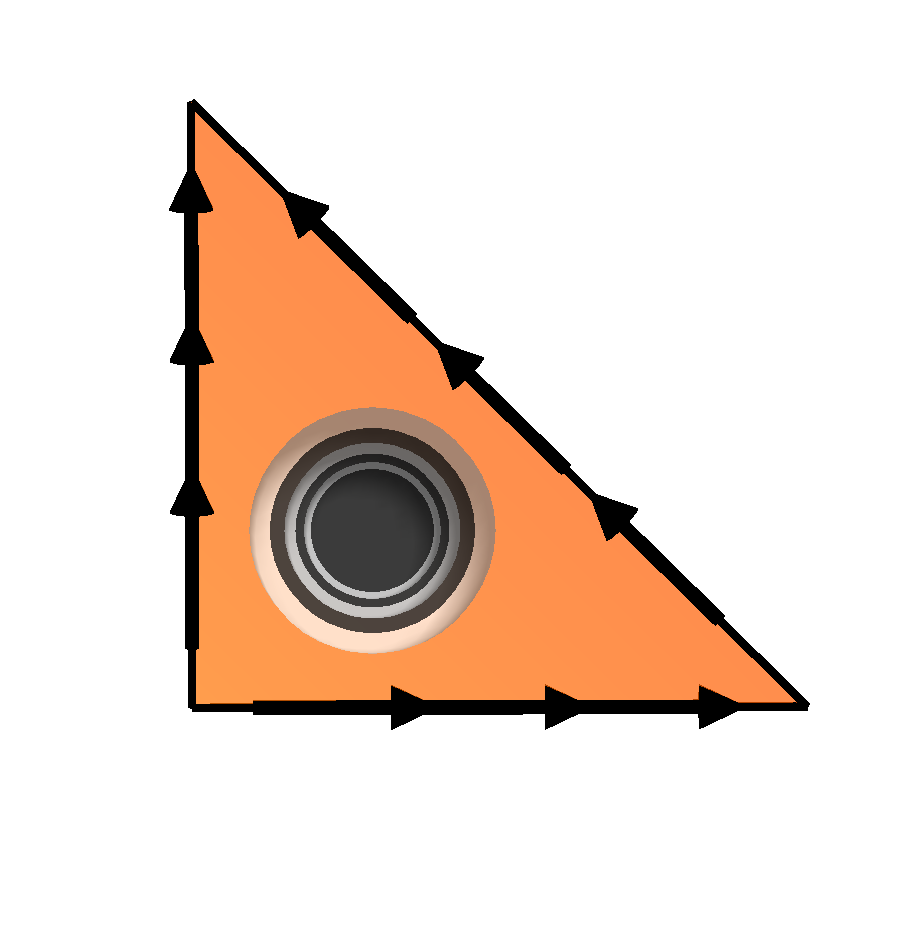
\includegraphics[width=\threefigs]{chapters/kirby-6/png/NED1_3_2d.png} \\
  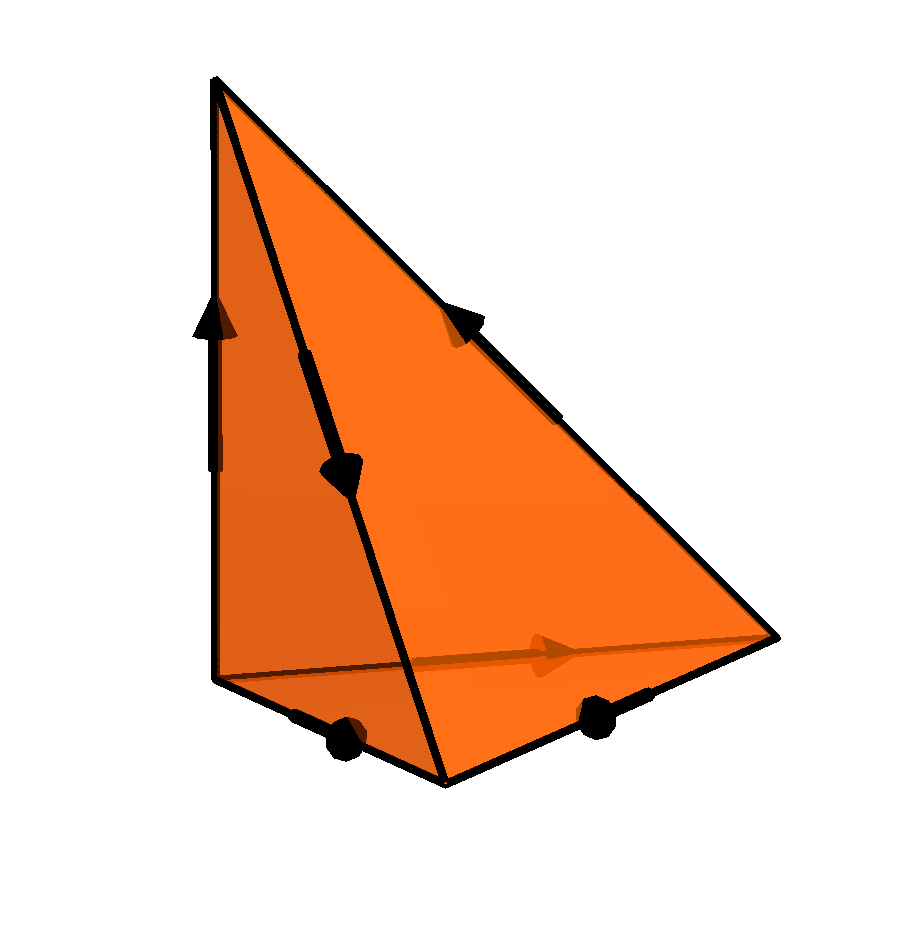
\includegraphics[width=\threefigs]{chapters/kirby-6/png/NED1_1_3d.png}
  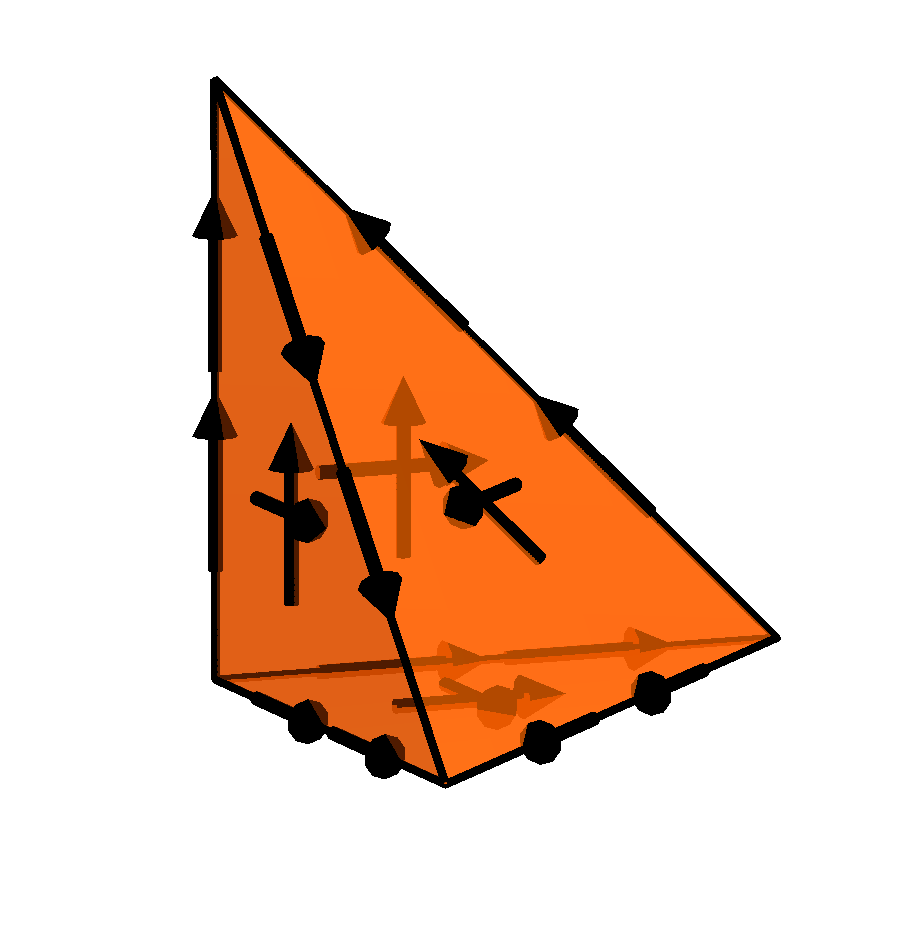
\includegraphics[width=\threefigs]{chapters/kirby-6/png/NED1_2_3d.png}
  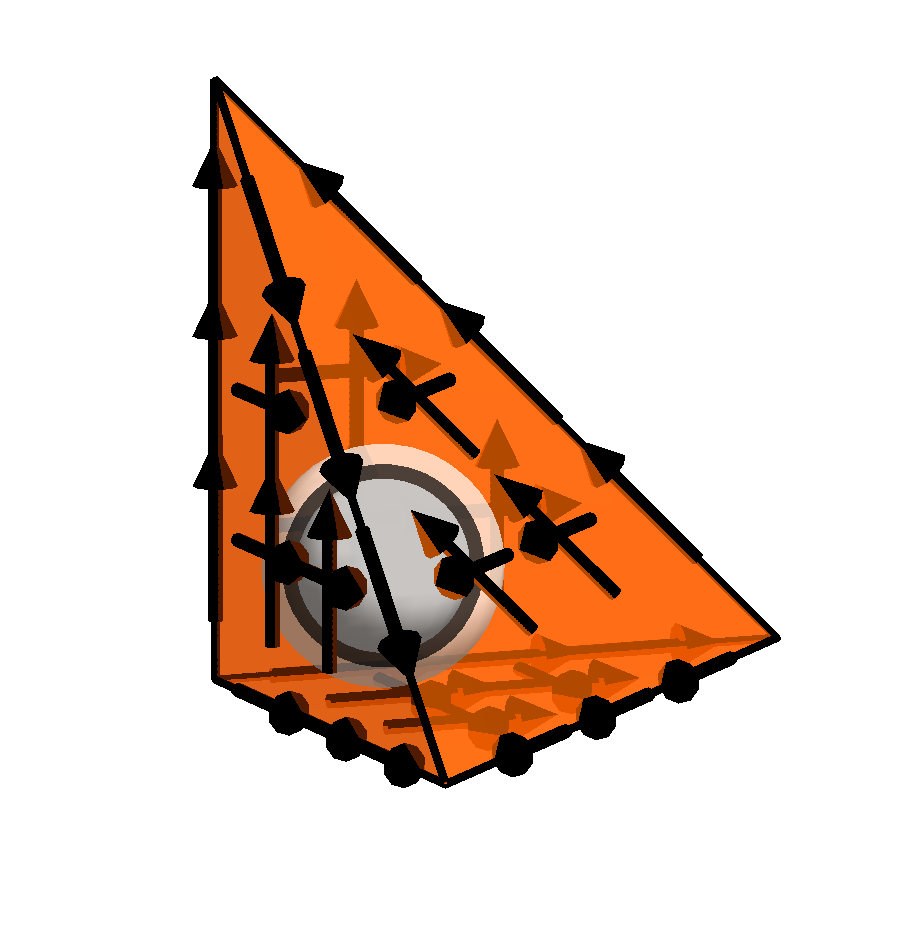
\includegraphics[width=\threefigs]{chapters/kirby-6/png/NED1_3_3d.png}
  \caption{Illustration of first, second and third degree \nedelec{}
    $\Hcurl$ elements of the first kind on triangles and
    tetrahedra. Note that these elements may be viewed as
    \emph{rotated} Raviart--Thomas elements. For the first degree
    \nedelec{} elements, the degrees of freedom are the average
    value over edges or, alternatively, the value of the tangential
    component at the midpoint of edges. Hence the term ``edge
    elements''.}
  \label{kirby-6:fig:ned1}
\end{figure}

Letting $\Pi_T^q$ denote the interpolation operator defined by the
degrees of freedom above, we have that \citep[Theorem 2]{Nedelec1980}
\begin{equation}
  ||u - \Pi_T^q u||_{H(\mathrm{curl})(T)} \leqslant C \, h_T^{q} |u|_{H^{q+1}(T)},
  \quad
  ||u - \Pi_T^q u||_{L^2(T)} \leqslant C \, h_T^{q} |u|_{H^{q}(T)}.
\end{equation}

\subsection{The $\Hcurl$ \nedelec{} element of the second kind}
\label{sec:nedelec:second}

\begin{definition}[\nedelec{} $\Hcurl$ element of the second kind]
  The \nedelec{} element of the second kind ($\mathrm{NED}^2_q$) is
  defined for $q = 1, 2, \dots$ in two dimensions by
  \begin{align}
    T &= \mathrm{triangle}, \\
    \CiarletSpace &= [\Poly{q}(T)]^2, \\
    \mathcal{L} &=
    \left \{
    \begin{array}{ll}
      \int_{e} v \cdot t \, p \ds,
      &\text{ for a set of basis functions }p \in \Poly{q}(e)
      \text{ for each edge } e,  \\
      \int_{T} v \cdot p \dx,
      &\text{ for a set of basis functions } p \in \mathrm{RT}_{q-1}(T),
      \text{ for } q \geqslant 2. \\
    \end{array}
    \right .
  \end{align}
  where $t$ is the edge tangent, and in three dimensions by
  \begin{align}
    T &= \mathrm{tetrahedron}, \\
    \CiarletSpace &= [\Poly{q}(T)]^3, \\
    \mathcal{L} &=
    \left \{
    \begin{array}{ll}
      \int_{e} v \cdot t \, p \, \mathrm{d}l,
      &\text{ for a set of basis functions } p \in \Poly{q}(e)
      \text{ for each edge } e, \\
      \int_{f} v \cdot p \ds,
      &\text{ for a set of basis functions } p \in \mathrm{RT}_{q-1}(f)
      \text{ for each face } f, \text{ for } q \geqslant 2 \\
      \int_{T} v \cdot p \dx,
      &\text{ for a set of basis functions } p \in \mathrm{RT}_{q-2}(T),
      \text{ for } q \geqslant 3.
    \end{array}
    \right .
  \end{align}
\end{definition}
The dimension of $\mathrm{NED^2}_q$ is
\begin{equation}
  n(q) = \left \{
    \begin{array}{ll}
      (q + 1)(q + 2), & T~\mathrm{triangle}, \\
      \frac{1}{2} (q + 1)(q + 2)(q + 3), & T~\mathrm{tetrahedron}. \\
    \end{array}
    \right.
\end{equation}

\begin{figure}
  \centering
  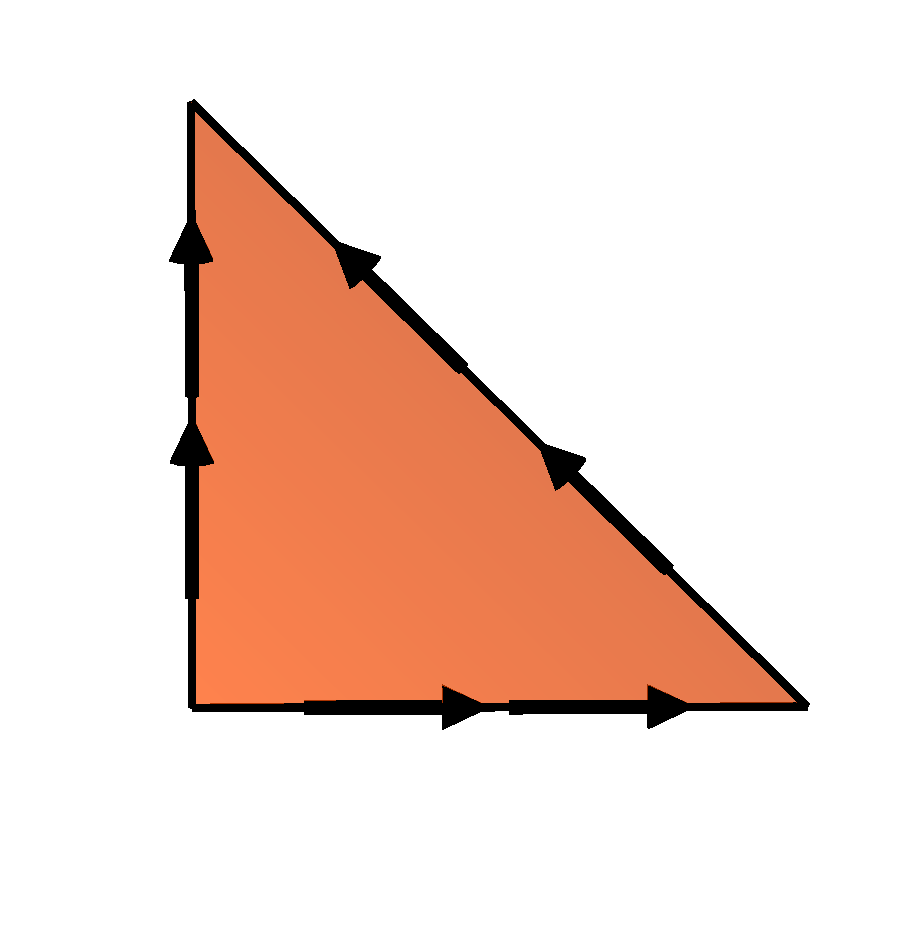
\includegraphics[width=\threefigs]{chapters/kirby-6/png/NED2_1_2d.png}
  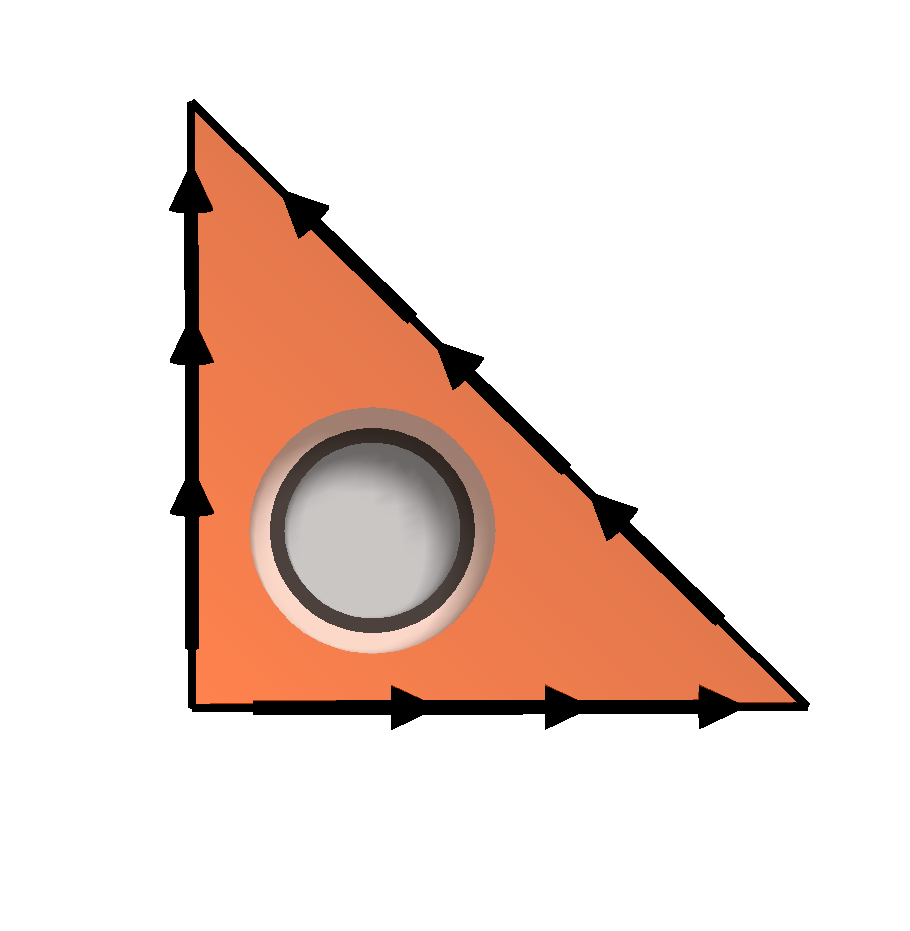
\includegraphics[width=\threefigs]{chapters/kirby-6/png/NED2_2_2d.png}
  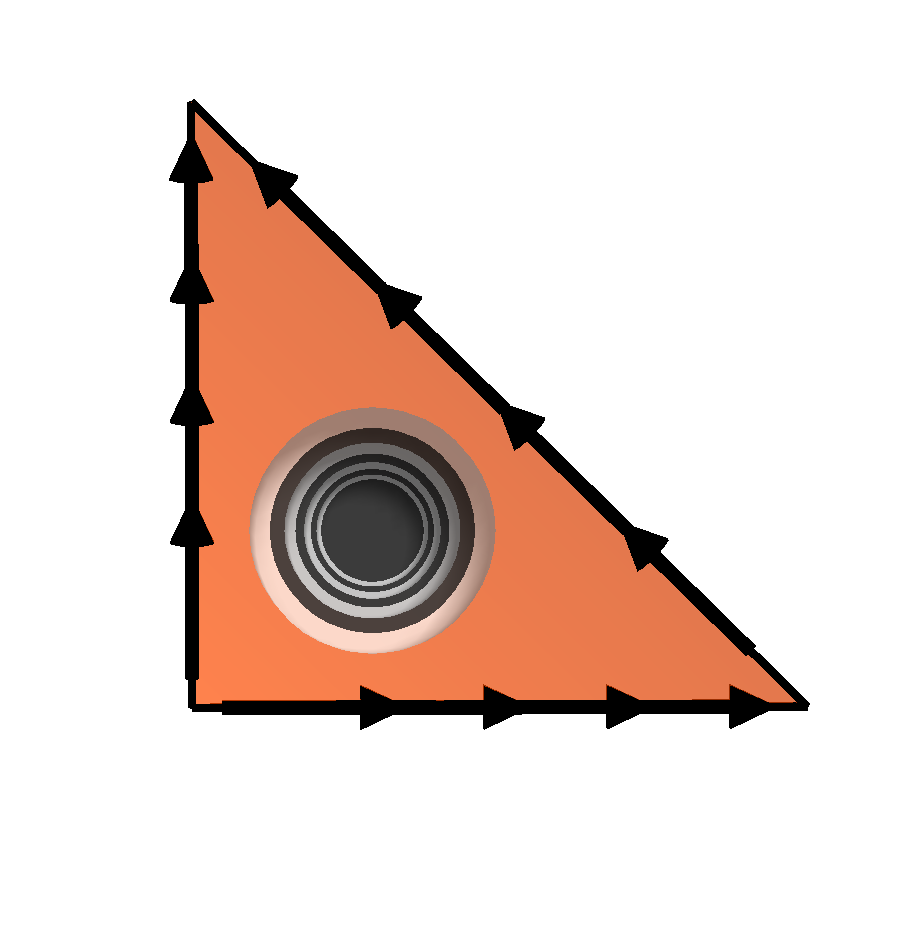
\includegraphics[width=\threefigs]{chapters/kirby-6/png/NED2_3_2d.png}
  \caption{Illustration of first, second and third degree \nedelec{}
    $\Hcurl$ elements of the second kind on triangles. Note that
    these elements may be viewed as \emph{rotated}
    Brezzi--Douglas--Marini elements.}
  \label{kirby-6:fig:ned2:tri}
\end{figure}

\begin{figure}
  \centering
  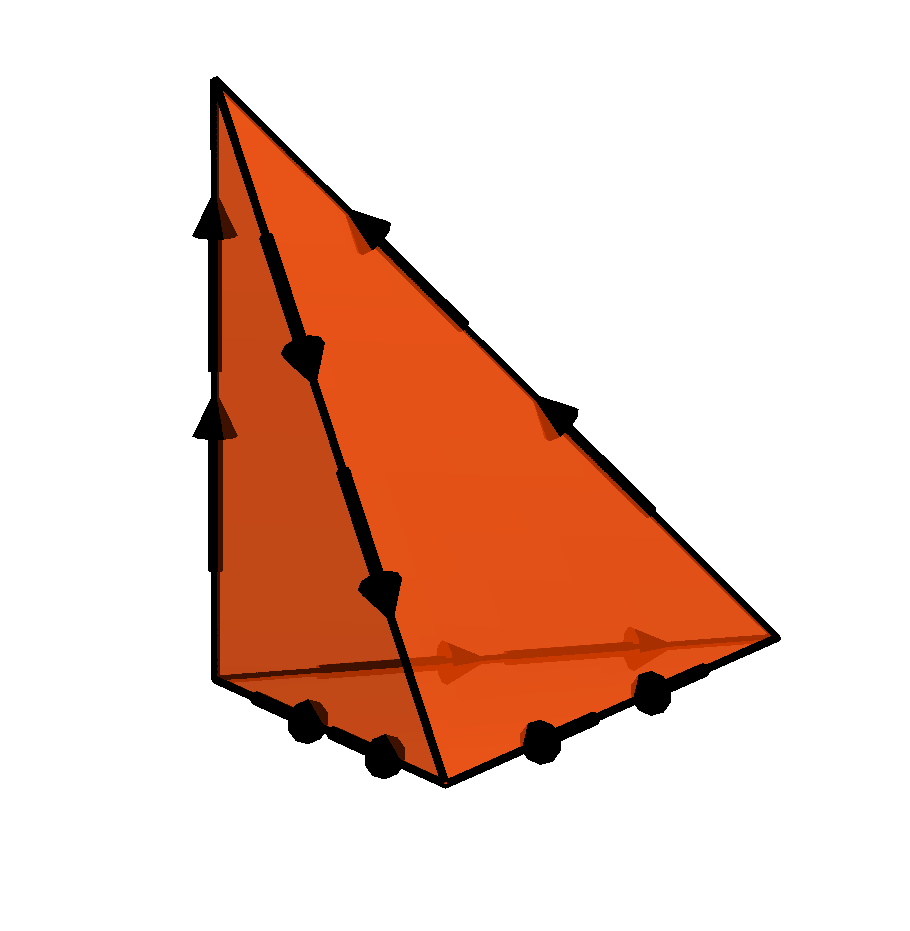
\includegraphics[width=\smallfig]{chapters/kirby-6/png/NED2_1_3d.png}
  \caption{Illustration of the first degree \nedelec{} $\Hcurl$
    elements of the second kind on tetrahedra.}
  \label{kirby-6:fig:ned2:tet}
\end{figure}

Letting $\Pi_T^q$ denote the interpolation operator defined by the
degrees of freedom above, we have that \citep[Proposition 3]{Nedelec1986}
\begin{equation}
  ||u - \Pi_T^q u||_{H(\mathrm{curl})(T)} \leqslant C \, h_T^{q} |u|_{H^{q+1}(T)}, \quad
  ||u - \Pi_T^q u||_{L^2(T)} \leqslant C \, h_T^{q+1} |u|_{H^{q+1}(T)}.
\end{equation}

%------------------------------------------------------------------------------
\section{$L^2$ elements}

By $L^2$ elements, one usually refers to finite element spaces where
the elements are not in $C^0$. Such elements naturally occur in mixed
formulations of the Poisson equation, Stokes flow, and
elasticity. Alternatively, such elements can be used for nonconforming
methods imposing\vadjust{\pagebreak} the desired \hbox{continuity} weakly instead of
directly. The discontinuous Galerkin (DG) methods provide a typical
example. In this case, the numerical flux of element facets is
assembled as part of the weak form; numerous variants of DG methods
have been defined with different numerical fluxes. DG methods were
originally developed for hyperbolic problems but have been
successfully applied to many elliptic and parabolic
problems. Moreover, the decoupling of each individual element provides
an increased opportunity for parallelism and $hp$-adaptivity.

\subsection{Discontinuous Lagrange}

\begin{definition}[Discontinuous Lagrange element]
  The discontinuous Lagrange element ($\mathrm{DG}_q$)
  is defined for $q = 0, 1, 2, \dots$ by
  \begin{align}
    T &\in \{ \mathrm{interval}{},
              \mathrm{triangle}{},
              \mathrm{tetrahedron}{}\}, \\
    \CiarletSpace &= \Poly{q}(T), \\
    \ell_i(v) &= v(x^i),
  \end{align}
  where $\{ x^i \}_{i=1}^{n(q)}$ is an enumeration of points in
  $T$ defined by
  \begin{equation}
    x =
    \left \{
    \begin{array}{lll}
      i/q,            & 0 \leqslant i \leqslant q,         & T~\mathrm{interval}, \\
      (i/q, j/q)      & 0 \leqslant i + j \leqslant q,     & T~\mathrm{triangle}, \\
      (i/q, j/q, k/q) & 0 \leqslant i + j + k \leqslant q, & T~\mathrm{tetrahedron}.
    \end{array}
    \right.
  \end{equation}
\end{definition}
The dimension of $\mathrm{DG}_q$ is
\begin{equation}
  n(q) =
    \left \{
    \begin{array}{ll}
      q + 1, & T~\mathrm{interval}, \\
      \frac{1}{2} (q + 1)(q + 2), & T~\mathrm{triangle}, \\
      \frac{1}{6} (q + 1)(q + 2)(q + 3), & T~\mathrm{tetrahedron}.
    \end{array}
    \right.
\end{equation}


Letting $\Pi_T^q$ denote the interpolation operator defined by the
degrees of freedom above, the interpolation properties of the $DG_q$
elements of degree $q$ are:
\begin{equation}
  ||u - \Pi_T^q u||_{L^2(T)} \leqslant C \, h_T^{q + 1} |u|_{H^{q+1}(T)}.
\end{equation}

%------------------------------------------------------------------------------
\section{$H^2$ finite elements}

The $H^2$ elements are commonly used in the approximation of
fourth-order problems, or for other spaces requiring at least $C^1$
continuity.  Due to the restrictive nature of the continuity
requirement, conforming elements are often of a high polynomial
degree, but lower degree nonconforming elements have proven to be
successful. Therefore, we here consider the conforming Argyris element
and the nonconforming Hermite and Morley elements.

\begin{figure}
\vspace*{-1pc}
  \centering
  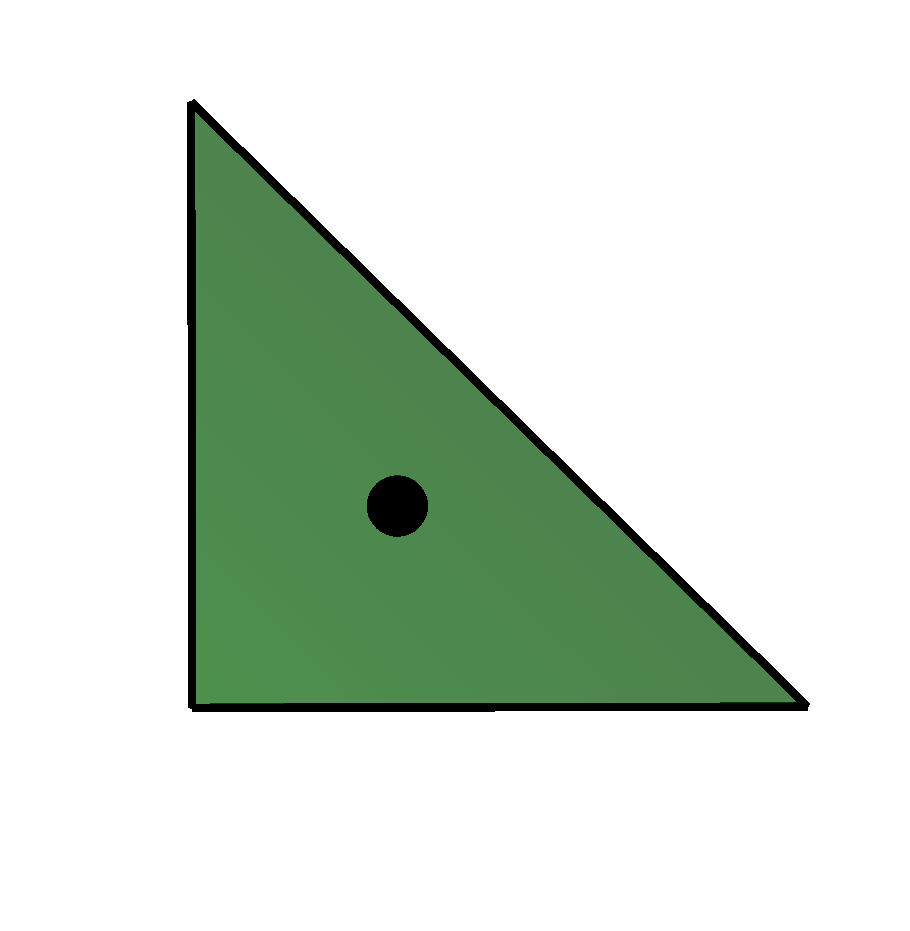
\includegraphics[width=\fourfigs]{chapters/kirby-6/png/DG0_2d.png}
  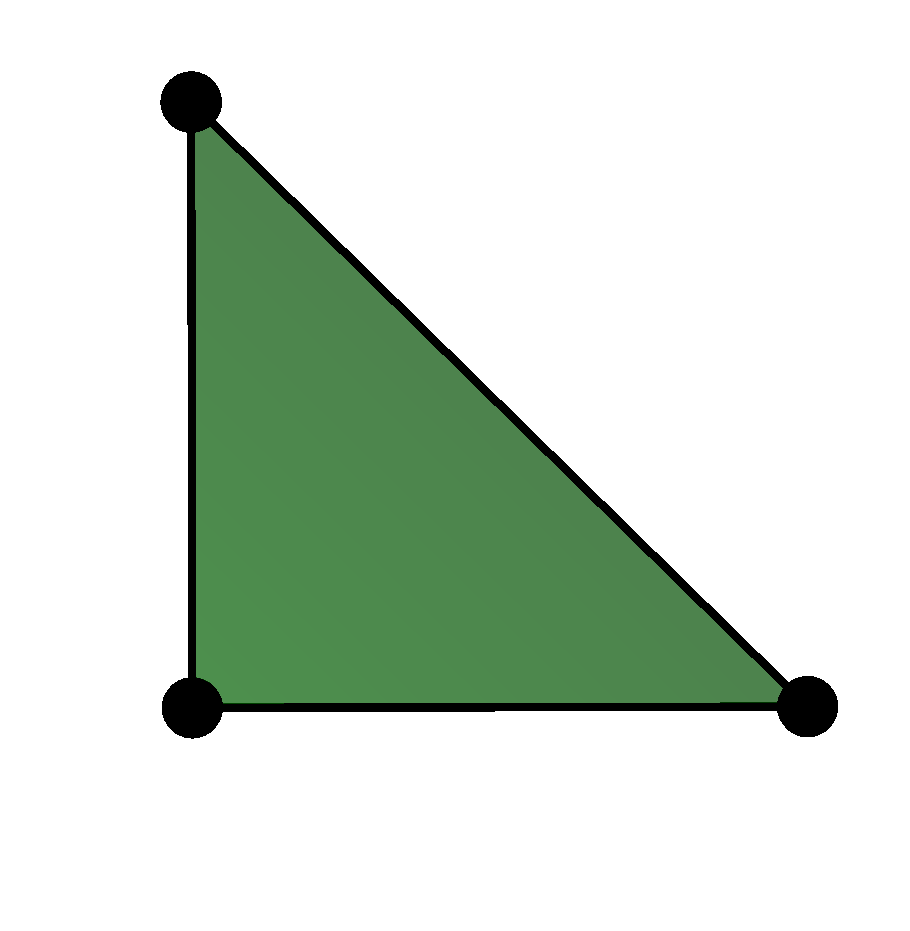
\includegraphics[width=\fourfigs]{chapters/kirby-6/png/DG1_2d.png}
  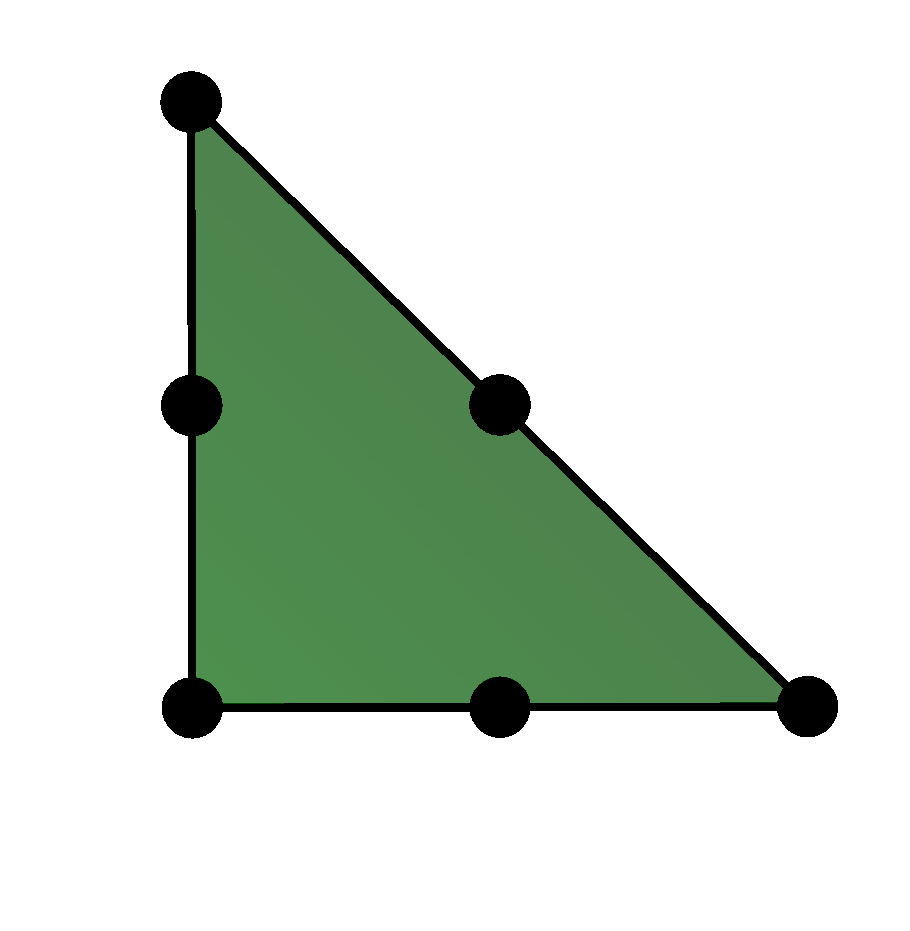
\includegraphics[width=\fourfigs]{chapters/kirby-6/png/DG2_2d.png}
  \includegraphics[width=\fourfigs]{chapters/kirby-6/png/DG3_2d.png} \\
  \includegraphics[width=\fourfigs]{chapters/kirby-6/png/DG0_3d.png}
  \includegraphics[width=\fourfigs]{chapters/kirby-6/png/DG1_3d.png}
  \includegraphics[width=\fourfigs]{chapters/kirby-6/png/DG2_3d.png}
  \includegraphics[width=\fourfigs]{chapters/kirby-6/png/DG3_3d.png} \\
  \caption{Illustration of the zeroth, first, second and third
    degree discontinuous Lagrange elements on triangles and
    tetrahedra. The degrees of freedom may be chosen arbitrarily as
    long as they span the dual space $\CiarletSpace'$. Here, the
    degrees of freedom have been chosen to be identical to those of
    the standard Lagrange finite element, with the difference that
    the degrees of freedom are viewed as \emph{internal} to the
    element.}
  \label{kirby-6:fig:dg}
  \vspace*{2pc}
\end{figure}

\begin{figure}
  \centering
  \includegraphics[width=\smallfig]{chapters/kirby-6/pdf/dgspace.pdf}
  \caption{All degrees of freedom of a discontinuous Lagrange finite
    element are internal to the element, which means that no global
    continuity is imposed by these elements. This is illustrated
    here for discontinuous quadratic Lagrange elements.}
\end{figure}


\subsection{The Argyris element}

The Argyris element \citep{ArgyrisFriedScharpf1968,Ciarlet2002} is
based on the space $\Poly{5}(T)$ of quintic polynomials over some triangle
$T$.  It can be pieced together with full $C^1$ continuity between
elements and $C^2$ continuity at the vertices of a triangulation.

\begin{definition}[Argyris element]
  The (quintic) Argyris element ($\mathrm{ARG}_5$) is defined by
  \begin{align}
    T &= \mathrm{triangle}, \\
    \CiarletSpace &= \Poly{5}(T), \\
    \mathcal{L} &=
    \left \{
    \begin{array}{ll}
      v(x^i),
      &\text{ for each vertex } x^i, \\
      \Grad v(x^i)_j,
      &\text{ for each vertex } x^i, \text{ and each component } j, \\
      D^2 v(x^i)_{jk},
      &\text{ for each vertex } x^i, \text{ and each component } jk, j \leqslant k, \\
      \Grad v(m^i) \cdot n,
      &\text{ for each edge midpoint } m^i. \\
    \end{array}
    \right .
  \end{align}
\end{definition}
The dimension of $\mathrm{ARG}_5$ is
\begin{equation}
  n = 21.
\end{equation}
Letting $\Pi_T$ denote the interpolation operator defined by the
degrees of freedom above, the interpolation properties of the
(quintic) Argyris elements are \citep[Chapter II.6]{Braess2007}:
\begin{equation}
  ||u - \Pi_T u||_{H^2(T)} \leqslant C \, h_T^{4} |u|_{H^6(T)}, \quad
  ||u - \Pi_T u||_{H^1(T)} \leqslant C \, h_T^{5} |u|_{H^6(T)}, \quad
  ||u - \Pi_T u||_{L^2(T)} \leqslant C \, h_T^{6} |u|_{H^6(T)}.
\end{equation}

\begin{figure}
  \centering
  \includegraphics[width=\smallfig]{chapters/kirby-6/png/ARG5_2d.png}
  \caption{The quintic Argyris triangle. The degrees of freedom are
    point evaluation, point evaluation of both first derivatives and
    point evaluation of all three second derivatives at the vertices
    of the triangle, and evaluation of the normal derivative at the
    midpoint of each edge.}
  \label{kirby-6:fig:argyris}
\end{figure}

The normal derivatives in the dual basis for the Argyris element
prevent it from being affine-interpolation equivalent. This prevents
the nodal basis from being constructed on a reference cell and
affinely mapped. Recent work by \citet{DominguezSayas2008} develops a
transformation that corrects this issue and requires less
computational effort than directly forming the basis on each cell in a
mesh. The Argyris element can be generalized to polynomial degrees
higher than quintic, still giving \( C^1 \) continuity with \( C^2 \)
continuity at the vertices \citep{SolinSegethDolevzel2004}.

\subsection{The Hermite element}

\looseness-1{}The Hermite element generalizes the classic cubic Hermite
interpolating polynomials on the line segment
\citep{Ciarlet2002}. Hermite-type elements appear in the finite
element literature almost from the beginning, appearing at least as
early as the classic paper by \citet{CiarletRaviart1972}. They have
long been known as useful $C^1$-nonconforming elements
\citep{Braess2007,Ciarlet2002}.  Under affine mappings, the Hermite
elements form \emph{affine-interpolation equivalent} families
\citep{BrennerScott2008}.

On the triangle, the space of cubic polynomials is ten-dimensional,
and the ten degrees of freedom for the Hermite element are point
evaluation at the triangle vertices and barycenter, together with the
components of the gradient evaluated at the vertices. The
generalization to tetrahedra is analogous.
\begin{definition}[Hermite element]
  The (cubic) Hermite element ($\mathrm{HER}$) is defined by
  \begin{align}
    T &\in \{ \mathrm{interval}{}, \mathrm{triangle}{}, \mathrm{tetrahedron}{}\}, \\
    \CiarletSpace &= \Poly{3}(T), \\
    \mathcal{L} &=
    \left \{
    \begin{array}{ll}
      v(x^i),
      &\text{ for each vertex } x^i, \\
      \Grad v(x^i)_j,
      &\text{ for each vertex } x^i, \text{ and each component } j, \\
      v(b),
      &\text{ for the barycenter $b$ (of the faces in 3D). }
    \end{array}
    \right.
  \end{align}
\end{definition}
The dimension of $\mathrm{HER}$ is
\begin{equation}
  n = \left \{
    \begin{array}{ll}
      10, & T~\mathrm{triangle}, \\
      20, & T~\mathrm{tetrahedron}.
    \end{array}
    \right.
\end{equation}

Letting $\Pi_T$ denote the interpolation operator defined by the
degrees of freedom above, the interpolation properties of the (cubic)
Hermite elements are:
\begin{equation}
  ||u - \Pi_T u||_{H^1(T)} \leqslant C \, h_T^{3} |u|_{H^4(T)}, \quad
  ||u - \Pi_T u||_{L^2(T)} \leqslant C \, h_T^{4} |u|_{H^4(T)}.
\end{equation}

\begin{figure}
  \centering
  \includegraphics[width=\twofigs]{chapters/kirby-6/png/HER_2d.png}
  \includegraphics[width=\twofigs]{chapters/kirby-6/png/HER_3d.png}
  \caption{The cubic Hermite triangle and tetrahedron. The degrees
    of freedom are point evaluation at the vertices and the
    barycenter, and evaluation of both first derivatives at the
    vertices.}
\end{figure}

Unlike the cubic Hermite functions on a line segment, the cubic
Hermite triangle and tetrahedron cannot be patched together in a fully
$C^1$ fashion. The cubic Hermite element can be extended to higher
degree \citep{BrennerScott2008}.


\subsection{The Morley element}

The Morley triangle defined in \citet{Morley1968} is a simple
$H^2$-nonconforming quadratic element that is used in fourth-degree
problems. The function space $\CiarletSpace$ is simply $\Poly{2}(T)$,
the six-dimensional space of quadratics. The degrees of freedom
consist of pointwise evaluation at each vertex and the normal
derivative at each edge midpoint. It is interesting to note that the
Morley triangle is neither $C^1$ nor even $C^0$, yet it is suitable
for fourth-order problems, and is the simplest known element for this
purpose.

The Morley element was first introduced to the engineering literature
by \citet{Morley1968,Morley1971}. In the mathematical literature,
\citet{LascauxLesaint1975} considered it in the context of the patch
test in a study of plate-bending elements. Recent applications of the
Morley element include \citet{HuangGuoShi2008,MinXu2006}.

\begin{definition}[Morley element]
  The (quadratic) Morley element ($\mathrm{MOR}$) is defined by
  \begin{align}
    T &= \mathrm{triangle}, \\
    \CiarletSpace &= \Poly{2}(T), \\
    \mathcal{L} &=
    \left \{
    \begin{array}{ll}
      v(x^i),
      &\text{ for each vertex } x^i, \\
      \Grad v(m^i) \cdot n,
      &\text{ for each edge midpoint } m^i. \\
    \end{array}
    \right.
  \end{align}
\end{definition}
The dimension of the Morley element is
\begin{equation}
  n = 6.
\end{equation}

Letting $\Pi_T$ denote the interpolation operator defined by the
degrees of freedom above, the interpolation properties of the
(quadratic) Morley elements are:
\begin{equation}
  ||u - \Pi_T u||_{H^1(T)} \leqslant C \, h_T^{2} |u|_{H^3(T)}, \quad
  ||u - \Pi_T u||_{L^2(T)} \leqslant C \, h_T^{3} |u|_{H^3(T)}.
\end{equation}

\begin{figure}
  \centering
  \includegraphics[width=\smallfig]{chapters/kirby-6/png/MOR_2d.png}
  \caption{The quadratic Morley triangle. The degrees of freedom are
    point evaluation at the vertices and evaluation of the normal
      derivative at the midpoint on each edge.}
\end{figure}

%------------------------------------------------------------------------------
\section{Enriching finite elements}

If $U, V$ are linear spaces, one can define a new linear space $W$ by
\begin{equation}
  W = \{ w = u + v \, : \, u \in U, v \in V \}.
\end{equation}
Here, we choose to call such a space $W$ an \emph{enriched space}.

The enrichment of a finite element space can lead to improved
stability properties, especially for mixed finite element
methods. Examples include the enrichment of the Lagrange element with
bubble functions for use with the Stokes equations or enriching the
Raviart--Thomas element for linear elasticity
\citep{ArnoldBrezziDouglas1984, ArnoldBrezziFortin1984}. Bubble
functions have since been used for many different applications. We
here define a \emph{bubble element} for easy reference. Notable
examples of the use of a bubble element include:
\paragraph{The MINI element for the Stokes equations.}
In the lowest degree case, the linear vector Lagrange element is
enriched with the cubic vector bubble element for the velocity
approximation \citep{ArnoldBrezziFortin1984}.\pagebreak

\paragraph{The PEERS element for weakly symmetric linear elasticity.}
Each row of the stress tensor is approximated by the lowest degree
Raviart--Thomas element enriched by the curl of the cubic bubble
element \citep{ArnoldBrezziDouglas1984}.

\begin{definition}[Bubble element]
  The bubble element ($B_q$) is defined for $q \geqslant (d+1)$ by
  \begin{align}
    T &\in \{ \mathrm{interval}{}, \mathrm{triangle}{}, \mathrm{tetrahedron}{}\}, \\
    \CiarletSpace &= \{ v \in \Poly{q}(T) \, : \, v|_{\partial T} = 0 \}, \\
    \ell_i(v) &= v(x^i), \quad i = 1, \dots, n(q).
  \end{align}
  where $\{x^i\}_{i=1}^{n(q)}$ is an enumeration of the
  points\footnote{Any other basis for the dual space of
    $\CiarletSpace$ will work just as well.} in $T$ defined by
  \begin{equation}
    x =\left \{\begin{array}{lll}
      (i + 1)/q,                   & 0 \leqslant i \leqslant q - 2,         & T~\mathrm{interval}, \\
      ((i+1)/q, (j+1)/q),          & 0 \leqslant i + j \leqslant q - 3,     & T~\mathrm{triangle}, \\
      ((i+1)/q, (j+1)/q, (k+1)/q), & 0 \leqslant i + j + k \leqslant q - 4, & T~\mathrm{tetrahedron}.
    \end{array}\right.
  \end{equation}
\end{definition}
The dimension of the Bubble element is
\begin{equation}
  n(q) =
    \left \{
    \begin{array}{ll}
      q - 1, & T~\mathrm{interval}, \\
      \frac{1}{2} (q - 2) (q - 1), & T~\mathrm{triangle}, \\
      \frac{1}{6} (q - 3) (q - 2) (q - 1), & T~\mathrm{tetrahedron}.
    \end{array}
    \right.
\end{equation}

%------------------------------------------------------------------------------
\section{Finite element exterior calculus}
It has recently been demonstrated that many of the finite elements
that have been discovered or invented over the years can be formulated
and analyzed in a common unifying framework as special cases of a more
general class of finite elements. This new framework is known as
\emph{finite element exterior calculus} and is summarized
in \citet{ArnoldFalkWinther2006}. In finite element exterior calculus,
two finite element spaces $\mathcal{P}_q\Lambda^k(T)$ and
$\mathcal{P}_q^-\Lambda^k(T)$ are defined for general simplices $T$ of
dimension $d \geqslant1$. The element $\mathcal{P}_q\Lambda^k(T)$ is
the space of polynomial differential $k$-forms\footnote{A differential
  $k$-form $\omega$ on a domain $\Omega$ maps each point $x \in
  \Omega$ to an alternating $k$-form $\omega_x$ on the tangent space
  $T_x(\Omega)$ of $\Omega$ at the point $x$. One can show that for
  $d=3$, the differential $k$-forms correspond to scalar-, vector-,
  vector-, and scalar-valued functions for $k=0,1,2,3$
  respectively. Thus, we may identify for example both
  $\mathcal{P}_q\Lambda^1$ and $\mathcal{P}_q\Lambda^2$ on a
  tetrahedron with the vector-valued polynomials of degree at most $q$
  on the tetrahedron.} on $T$ with degrees of freedom chosen to ensure
continuity of the trace on facets. When these elements are interpreted
as regular elements, by a suitable identification between differential
$k$-forms and scalar- or vector-valued functions, one obtains a series
of well-known elements for $0\leqslant k \leqslant d \leqslant 3$. In
Table~\ref{tab:feec}, we summarize the relation between these elements
and the elements presented above in this chapter\footnote{The finite
  elements $\mathcal{P}_q\Lambda^k(T)$ and
  $\mathcal{P}_q^-\Lambda^k(T)$ have been implemented for general
  values of $k$, $q$ and $d=1,2,3,4,\ldots$ as part of the FEniCS
  \emph{Exterior} package available from
  \url{http://launchpad.net/exterior}.}.

\begin{table}
  \centering
  \begin{tabular}{ccc}
    $\mathcal{P}_q \Lambda^k$ & & $\mathcal{P}^-_q \Lambda^k$ \\
    \\
    $\begin{array}{cccc}
      \toprule
      k & d = 1 & d = 2 & d = 3 \\
      \midrule
      0 & \mathrm{CG}_q & \mathrm{CG}_q  & \mathrm{CG}_q \\
      1 & \mathrm{DG}_q & \mathrm{NED}^{\mathrm{2, curl}}_q & \mathrm{NED}^{\mathrm{2, curl}}_q \\
      2 & \mbox{---} & \mathrm{DG}_q & \mathrm{BDM}_q \\
      3 & \mbox{---} & \mbox{---} & \mathrm{DG}_q \\
      \bottomrule
    \end{array}$    & \quad &
    $\begin{array}{cccc}
      \toprule
      k & d = 1 & d = 2 & d = 3 \\
      \midrule
      0 & \mathrm{CG}_q & \mathrm{CG}_q  & \mathrm{CG}_q \\
      1 & \mathrm{DG}_{q-1} & \mathrm{NED}^{\mathrm{1, curl}}_q & \mathrm{NED}^{\mathrm{1, curl}}_q \\
      2 & \mbox{---}  &  \mathrm{DG}_{q-1} & \mathrm{RT}_q \\
      3 & \mbox{---}  & \mbox{---} & \mathrm{DG}_{q-1} \\
      \bottomrule
    \end{array}$
  \end{tabular}
  \caption{Relationships between the finite elements $\mathcal{P}_q
    \Lambda^k$ and $\mathcal{P}^-_q \Lambda^k$ defined by finite
    element exterior calculus and their more traditional
    counterparts using the numbering and labeling of this chapter.}
  \label{tab:feec}
\end{table}

%------------------------------------------------------------------------------
\section{Summary}

In the table below, we summarize the list of elements discussed in
this chapter. For brevity, we include element degrees only up to and
including $q = 3$. For higher degree elements, we refer to the script
\emp{dolfin-plot} available as part of FEniCS, which can be used to
easily plot the degrees of freedom for a wide range of elements:
\begin{bash}
$ dolfin-plot BDM tetrahedron 3
$ dolfin-plot N1curl triangle 4
$ dolfin-plot CG tetrahedron 5
\end{bash}
Elements indicated with at $(*)$ in the table below are fully
supported by FEniCS.

% Use for vertical centering of table entries, strange thing is we
% need at least three of these in the table to get horisontal alignment.
{
\newcolumntype{S}{>{\centering\arraybackslash}m{2.0cm}}
\newcolumntype{T}{>{\centering\arraybackslash}m{1.4cm}}
    \small
    \centering
   \begin{longtable}{p{4.1cm}SSTp{4cm}}
     \toprule
     Element family & Notation & Illustration & Dimension & Description \\
     \hline
     (Quintic) Argyris             & $\mathrm{ARG}_5$   (2D) & \elmfig{ARG5_2d}   & $n = 21$ &
     \elmdesc{$\Poly{5}$ (scalar); $3$ point values, $3 \times 2$ derivatives, $3\times 3$ second derivatives, $3$ directional derivatives}
     \hline
     Arnold--Winther               & $\mathrm{AW}$      (2D) & \elmfig{AW_2d}     & $n = 24$ &
     \elmdesc{$\Poly{3}(T; \mathbb{S})$ (matrix) with linear divergence; $3 \times 3$ point values, $12$ normal components, $3$ interior moments}
     \hline
     Brezzi--Douglas--Marini $(*)$ & $\mathrm{BDM}_1$   (2D) & \elmfig{BDM1_2d}   & $n = 6$ &
     \elmdesc{$[\Poly{1}]^2$ (vector); $6$ normal components}
     \hline
     Brezzi--Douglas--Marini $(*)$ & $\mathrm{BDM}_2$   (2D) & \elmfig{BDM2_2d}   & $n = 12$ &
     \elmdesc{$[\Poly{2}]^2$ (vector); $9$ normal components, $3$ interior moments}
     \hline
     Brezzi--Douglas--Marini $(*)$ & $\mathrm{BDM}_3$   (2D) & \elmfig{BDM3_2d}   & $n = 20$ &
     \elmdesc{$[\Poly{3}]^2$ (vector); $12$ normal components, $8$ interior moments}
     \hline
     Brezzi--Douglas--Marini $(*)$ & $\mathrm{BDM}_1$   (3D) & \elmfig{BDM1_3d}   & $n = 12$ &
     \elmdesc{$[\Poly{1}]^3$ (vector); $12$ normal components}
     \hline
     Brezzi--Douglas--Marini $(*)$   & $\mathrm{BDM}_2$   (3D) & \elmfig{BDM2_3d}   & $n = 30$ &
     \elmdesc{$[\Poly{2}]^3$ (vector); $24$ normal components, $6$ interior moments}
     \hline
     Brezzi--Douglas--Marini $(*)$   & $\mathrm{BDM}_3$   (3D) & \elmfig{BDM3_3d}   & $n = 60$ &
     \elmdesc{$[\Poly{3}]^3$ (vector); $40$ normal components, $20$ interior moments}
     \hline
     Crouzeix--Raviart       $(*)$   & $\mathrm{CR}_1$    (2D) & \elmfig{CR1_2d}    & $n = 3$ &
     \elmdesc{$\Poly{1}$ (scalar); $3$ point values}
     \hline
     Crouzeix--Raviart       $(*)$   & $\mathrm{CR}_1$    (3D) & \elmfig{CR1_3d}    & $n = 4$ &
     \elmdesc{$\Poly{1}$ (scalar); $4$ point values}
     \hline
     Discontinuous Lagrange  $(*)$   & $\mathrm{DG}_0$    (2D) & \elmfig{DG0_2d}    & $n = 1$ &
     \elmdesc{$\Poly{0}$ (scalar); $1$ point value}
     \hline
     Discontinuous Lagrange  $(*)$   & $\mathrm{DG}_1$    (2D) & \elmfig{DG1_2d}    & $n = 3$ &
     \elmdesc{$\Poly{1}$ (scalar); $3$ point values}
     \hline
     Discontinuous Lagrange  $(*)$   & $\mathrm{DG}_2$    (2D) & \elmfig{DG2_2d}    & $n = 6$ &
     \elmdesc{$\Poly{2}$ (scalar); $6$ point values}
     \hline
     Discontinuous Lagrange  $(*)$   & $\mathrm{DG}_3$    (2D) & \elmfig{DG3_2d}    & $n = 10$ &
     \elmdesc{$\Poly{3}$ (scalar); $10$ point values}
     \hline
     Discontinuous Lagrange  $(*)$   & $\mathrm{DG}_0$    (3D) & \elmfig{DG0_3d}    & $n = 1$ &
     \elmdesc{$\Poly{0}$ (scalar); $1$ point value}
     \hline
     Discontinuous Lagrange  $(*)$   & $\mathrm{DG}_1$    (3D) & \elmfig{DG1_3d}    & $n = 4$ &
     \elmdesc{$\Poly{1}$ (scalar); $4$ point values}
     \hline
     Discontinuous Lagrange  $(*)$   & $\mathrm{DG}_2$    (3D) & \elmfig{DG2_3d}    & $n = 10$ &
     \elmdesc{$\Poly{2}$ (scalar); $10$ point values}
     \hline
     Discontinuous Lagrange  $(*)$   & $\mathrm{DG}_3$    (3D) & \elmfig{DG3_3d}    & $n = 20$ &
     \elmdesc{$\Poly{3}$ (scalar); $20$ point values}
     \hline
     (Cubic) Hermite              & $\mathrm{HER}$     (2D) & \elmfig{HER_2d}    & $n = 10$ &
     \elmdesc{$\Poly{3}$ (scalar); $4$ point values, $3 \times 2$ derivatives}
     \hline
     (Cubic) Hermite              & $\mathrm{HER}$     (3D) & \elmfig{HER_3d}    & $n = 20$ &
     \elmdesc{$\Poly{3}$ (scalar); $8$ point values, $4 \times 3$ derivatives}
     \hline
     Lagrange                $(*)$ & $\mathrm{CG}_1$    (2D) & \elmfig{CG1_2d}    & $n = 3$ &
     \elmdesc{$\Poly{1}$ (scalar); $3$ point values}
     \hline
     Lagrange                $(*)$ & $\mathrm{CG}_2$    (2D) & \elmfig{CG2_2d}    & $n = 6$ &
     \elmdesc{$\Poly{2}$ (scalar); $6$ point values}
     \hline
     Lagrange                $(*)$ & $\mathrm{CG}_3$    (2D) & \elmfig{CG3_2d}    & $n = 10$ &
     \elmdesc{$\Poly{3}$ (scalar); $10$ point values}
     \hline
     Lagrange                $(*)$ & $\mathrm{CG}_1$    (3D) & \elmfig{CG1_3d}    & $n = 4$ &
     \elmdesc{$\Poly{1}$ (scalar); $4$ point values}
     \hline
     Lagrange                $(*)$ & $\mathrm{CG}_2$    (3D) & \elmfig{CG2_3d}    & $n = 10$ &
     \elmdesc{$\Poly{2}$ (scalar); $10$ point values}
     \hline
     Lagrange                $(*)$ & $\mathrm{CG}_3$    (3D) & \elmfig{CG3_3d}    & $n = 20$ &
     \elmdesc{$\Poly{2}$ (scalar); $20$ point values}
     \hline
     Mardal--Tai--Winther         & $\mathrm{MTW}$     (2D) & \elmfig{MTW_2d}    & $n = 9$ &
     \elmdesc{$[\Poly{2}]^2$ (vector); with constant divergence and linear normal components; $6$ moments of normal components, $3$ moments of tangential components}
     \hline
     (Quadratic) Morley           & $\mathrm{MOR}$     (2D) & \elmfig{MOR_2d}    & $n = 6$ &
     \elmdesc{$\Poly{2}$ (scalar); $3$ point values, $3$ directional derivatives}
     \hline
     \nedelec{} 1st kind $\Hcurl$ $(*)$ & $\mathrm{NED}^1_1$ (2D) & \elmfig{NED1_1_2d} & $n = 3$ &
     \elmdesc{$[\Poly{0}]^2 + S_1$ (vector); $3$ tangential components}
     \hline
     \nedelec{} 1st kind $\Hcurl$ $(*)$ & $\mathrm{NED}^1_2$ (2D) & \elmfig{NED1_2_2d} & $n = 8$ &
     \elmdesc{$[\Poly{1}]^2 + S_2$ (vector); $6$ tangential components, $2$ interior moments}
     \hline
     \nedelec{} 1st kind $\Hcurl$ $(*)$ & $\mathrm{NED}^1_3$ (2D) & \elmfig{NED1_3_2d} & $n = 15$ &
     \elmdesc{$[\Poly{2}]^2 + S_3$ (vector); $9$ tangential components, $6$ interior moments}
     \hline
     \nedelec{} 1st kind $\Hcurl$ $(*)$ & $\mathrm{NED}^1_1$ (3D) & \elmfig{NED1_1_3d} & $n = 6$ &
     \elmdesc{$[\Poly{0}]^3 + S_1$ (vector); $6$ tangential components}
     \hline
     \nedelec{} 1st kind $\Hcurl$ $(*)$ & $\mathrm{NED}^1_2$ (3D) & \elmfig{NED1_2_3d} & $n = 20$ &
     \elmdesc{$[\Poly{1}]^3 + S_2$ (vector); $20$ tangential components}
     \hline
     \nedelec{} 1st kind $\Hcurl$ $(*)$ & $\mathrm{NED}^1_3$ (3D) & \elmfig{NED1_3_3d} & $n = 45$ &
     \elmdesc{$[\Poly{2}]^3 + S_3$ (vector); $42$ tangential components, $3$ interior moments}
     \hline
     \nedelec{} 2nd kind $\Hcurl$ $(*)$ & $\mathrm{NED}^2_1$ (2D) & \elmfig{NED2_1_2d} & $n = 6$ &
     \elmdesc{$[\Poly{1}]^2$ (vector); $6$ tangential components}
     \hline
     \nedelec{} 2nd kind $\Hcurl$ $(*)$ & $\mathrm{NED}^2_2$ (2D) & \elmfig{NED2_2_2d} & $n = 12$ &
     \elmdesc{$[\Poly{2}]^2$ (vector); $9$ tangential components, $3$ interior moments}
     \hline
     \nedelec{} 2nd kind $\Hcurl$ $(*)$ & $\mathrm{NED}^2_3$ (2D) & \elmfig{NED2_3_2d} & $n = 20$ &
     \elmdesc{$[\Poly{3}]^2$ (vector); $12$ tangential components, $8$ interior moments}
     \hline
     \nedelec{} 2nd kind $\Hcurl$ $(*)$ & $\mathrm{NED}^2_1$ (3D) & \elmfig{NED2_1_3d} & $n = 12$ &
     \elmdesc{$[\Poly{1}]^3$ (vector); $12$ tangential components}
     \hline
     Raviart--Thomas         $(*)$ & $\mathrm{RT}_1$    (2D) & \elmfig{RT1_2d}    & $n = 3$ &
     \elmdesc{$[\Poly{0}]^2 + x \Poly{0}$ (vector); $3$ normal components}
     \hline
     Raviart--Thomas         $(*)$ & $\mathrm{RT}_2$    (2D) & \elmfig{RT2_2d}    & $n = 8$ &
     \elmdesc{$[\Poly{1}]^2 + x \Poly{1}$ (vector); $6$ normal components, $2$ interior moments}
     \hline
     Raviart--Thomas         $(*)$ & $\mathrm{RT}_3$    (2D) & \elmfig{RT3_2d}    & $n = 15$ &
     \elmdesc{$[\Poly{2}]^2 + x \Poly{2}$ (vector); $9$ normal components, $6$ interior moments}
     \hline
     Raviart--Thomas         $(*)$ & $\mathrm{RT}_1$    (3D) & \elmfig{RT1_3d}    & $n = 4$ &
     \elmdesc{$[\Poly{0}]^3 + x \Poly{0}$ (vector); $4$ normal components}
     \hline
     Raviart--Thomas         $(*)$ & $\mathrm{RT}_2$    (3D) & \elmfig{RT2_3d}    & $n = 15$ &
     \elmdesc{$[\Poly{1}]^3 + x \Poly{1}$ (vector); $12$ normal components, $3$ interior moments}
     \hline
     Raviart--Thomas         $(*)$ & $\mathrm{RT}_3$    (3D) & \elmfig{RT3_3d}    & $n = 36$ &
     \elmdesc{$[\Poly{2}]^3 + x \Poly{2}$ (vector); $24$ normal components, $12$ interior moments}
     \bottomrule
   \end{longtable}
}
